\documentclass[11pt,a4paper]{article}
\usepackage[utf8]{inputenc}
\usepackage[T1]{fontenc}
\usepackage[spanish,es-noquoting]{babel}
\usepackage{lmodern}
\usepackage{geometry}
\usepackage{graphicx}
\usepackage{array}
\usepackage{tabularx}
\usepackage{longtable}
\usepackage{booktabs}
\usepackage{multirow}
\usepackage{float}
\usepackage{caption}
\usepackage{subcaption}
\usepackage{enumitem}
\usepackage{hyperref}
\usepackage{xcolor}
\usepackage{fancyhdr}
\usepackage{titlesec}
\usepackage{setspace}
\usepackage{microtype}
\usepackage{placeins}

\geometry{margin=2.5cm}
\setlength{\parindent}{0pt}
\setlength{\parskip}{0.55em}
\setstretch{1.08}
\graphicspath{{_tfg_pdf_assets/}}
\hypersetup{
  colorlinks=true,
  linkcolor=blue!60!black,
  urlcolor=blue!60!black,
  citecolor=blue!60!black,
  pdftitle={TFG 3ª Entrega - La Galana Manager},
  pdfauthor={Manuel Rodríguez Méndez}
}
\urlstyle{same}

\pagestyle{fancy}
\fancyhf{}
\fancyhead[L]{Memoria - Casa Rural La Galana}
\fancyhead[R]{\thepage}
\fancyfoot[C]{}
\renewcommand{\headrulewidth}{0.4pt}
\renewcommand{\footrulewidth}{0pt}

\titleformat{\section}
  {\normalfont\Large\bfseries}{\thesection.}{0.5em}{}
\titleformat{\subsection}
  {\normalfont\large\bfseries}{\thesubsection.}{0.5em}{}
\titleformat{\subsubsection}
  {\normalfont\normalsize\bfseries}{\thesubsubsection.}{0.5em}{}
\titleformat{\paragraph}[block]
  {\normalfont\normalsize\bfseries}{\theparagraph.}{0.5em}{}
\titlespacing*{\paragraph}{0pt}{0.8em}{0.35em}

\newcolumntype{Y}{>{\raggedright\arraybackslash}X}
\newcolumntype{L}{>{\raggedright\arraybackslash}p{0.18\textwidth}}

\captionsetup[figure]{font=small,labelfont=bf,justification=raggedright,singlelinecheck=false}
\captionsetup[table]{font=small,labelfont=bf,justification=raggedright,singlelinecheck=false}

\begin{document}

\begin{titlepage}
  \thispagestyle{empty}
  \centering
  \vspace*{-1.0cm}
  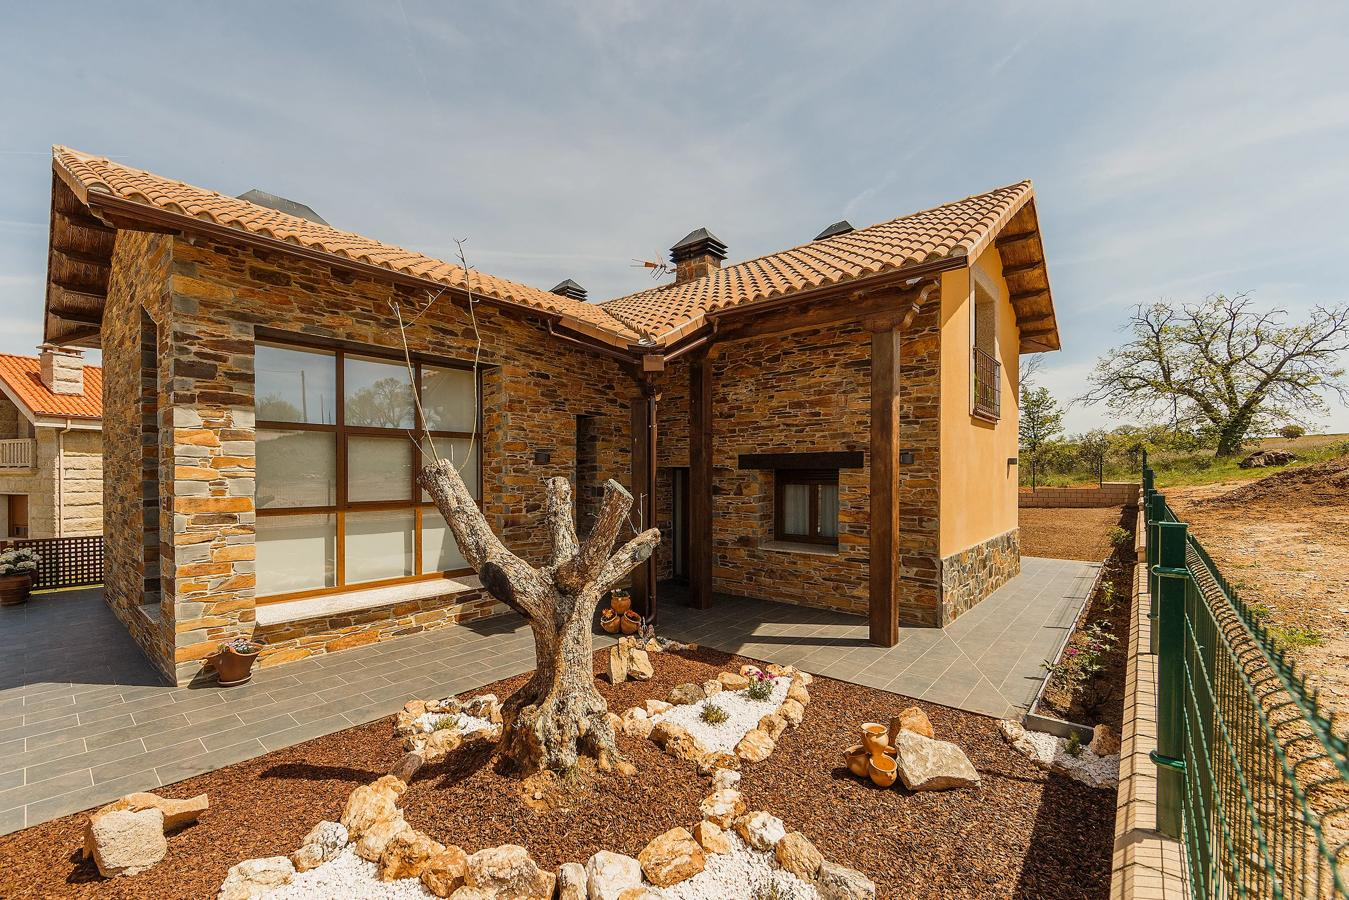
\includegraphics[width=\textwidth,height=0.58\textheight,keepaspectratio]{page-01-image-1.jpeg}

  \vspace{1.1cm}
  {\Huge\bfseries LA GALANA MANAGER\par}
  \vspace{0.35cm}
  {\Large Memoria del proyecto intermodular\par}

  \vspace{1.1cm}
  \begin{tabular}{@{}ll@{}}
    \textbf{Autor:} & Manuel Rodríguez Méndez \\
    \textbf{Ciclo:} & Desarrollo de Aplicaciones Web (DAW) \\
    \textbf{Tutor:} & Santiago Blanco Arenal \\
    \textbf{Tecnologías:} & React, Vite, Tailwind CSS, Supabase y react-calendar
  \end{tabular}

  \vfill
\end{titlepage}

\pagenumbering{arabic}
\setcounter{page}{2}
\setcounter{tocdepth}{4}
\setcounter{secnumdepth}{4}
\setcounter{section}{-1}

\section{Presentación}

\subsection{Portada}
La portada identifica el proyecto, el autor, el ciclo formativo, el tutor, la fecha de actualización y las tecnologías principales utilizadas en la aplicación.

\subsection{Agradecimientos y dedicatoria}
Agradezco el apoyo recibido durante el desarrollo del proyecto y el material gráfico de Casa Rural La Galana, ya que las fotografías reales han permitido construir una aplicación más fiel al alojamiento y más útil para el usuario final.

\subsection{Índice del documento}
\tableofcontents

\subsection{Lista de imágenes}
\begin{longtable}{|>{\bfseries}p{1.2cm}|p{3.8cm}|p{9.6cm}|}
\caption{Lista de imágenes}\label{tab:lista-imagenes}\\
\hline
Nº & Imagen & Descripción \\
\hline
\endfirsthead
\hline
Nº & Imagen & Descripción \\
\hline
\endhead
1 & Portada de Casa Rural La Galana & Imagen real utilizada como presentación visual del proyecto. \\
2 & Diagrama de Gantt actualizado & Resumen temporal del avance del proyecto. \\
  3 & Diagrama relacional revisado & Modelo de datos revisado. \\
4 & Diagrama de clases / componentes & Relación de componentes reales de la aplicación. \\
5 & Casos de uso del Visitante & Diagrama de interacción del visitante. \\
6 & Casos de uso del Cliente & Diagrama de interacción del cliente. \\
7 & Casos de uso del Administrador & Diagrama de interacción del administrador. \\
8 & Flujo de reserva actual & Secuencia actual del proceso de reserva. \\
\hline
\end{longtable}

\subsection{Lista de tablas}
\begin{longtable}{|>{\bfseries}p{1.2cm}|p{4.7cm}|p{7.5cm}|}
\caption{Lista de tablas}\label{tab:lista-tablas}\\
\hline
Nº & Tabla & Apartado \\
\hline
\endfirsthead
\hline
Nº & Tabla & Apartado \\
\hline
\endhead
1 & Comparación entre documentación anterior y aplicación actual & 1.2 / 4.1 \\
2 & Recursos necesarios & 2 \\
3 & Planificación actualizada & 3.2 \\ 	
4 & Modelo de datos revisado & 4.2 \\
5 & Casos de uso actualizados & 4.3.1 \\
6 & Pruebas realizadas & 5.1 \\
\hline
\end{longtable}

\section{Estudio del problema y análisis del sistema}

\subsection{Introducción}
El proyecto consiste en desarrollar una aplicación web para Casa Rural La Galana. La documentación anterior planteaba una herramienta de gestión amplia, orientada a disponibilidad, reservas, clientes, temporadas, extras, bloqueos, exportaciones y administración. La aplicación actual ya combina una web pública para visitantes con un panel administrativo que permite gestionar reservas, usuarios, temporadas, extras, galería y documentos de reserva.

Esta memoria toma como base el índice oficial facilitado y actualiza el contenido anterior para que refleje el estado real del proyecto. Se diferencian claramente tres niveles: funcionalidades implementadas, funcionalidades parcialmente implementadas y funcionalidades previstas para futuras versiones.

\subsection{Descripción de la aplicación. Motivación. Finalidad}
La finalidad actual del sistema es ofrecer una web moderna para Casa Rural La Galana, mejorar su presencia digital y facilitar que un visitante pueda conocer la casa, ver fotografías reales, consultar disponibilidad, seleccionar fechas, añadir extras y guardar una solicitud de reserva en Supabase.

A diferencia de la documentación anterior, la aplicación actual ya incorpora una parte importante de la gestión interna. El panel administrativo permite consultar indicadores, administrar reservas, gestionar imágenes de la galería, mantener usuarios, configurar extras y definir precios por temporada.

\begin{table}[H]
\centering
\small
\begin{tabularx}{\textwidth}{|p{2.6cm}|p{3.2cm}|p{3.2cm}|p{5.2cm}|}
\hline
\textbf{Área} & \textbf{Lo escrito en el documento anterior} & \textbf{Lo existente ahora en la aplicación} & \textbf{Cambio aplicado en esta memoria} \\
\hline
Web pública & Página inicial informativa y llamadas a consultar disponibilidad. & Home completa con hero visual, información, galería destacada, reserva y footer. & Se actualiza como funcionalidad implementada. \\
\hline
Galería & Galería prevista de imágenes. & Carrusel 3D, página \texttt{/galeria}, categorías dinámicas y almacenamiento de imágenes en Supabase Storage. & Se documenta como módulo público y administrable. \\
\hline
Cómo llegar/contacto & Mapa interactivo y contacto rápido. & Enlaces a Google Maps, teléfono y WhatsApp desde la navegación. & Se ajusta a la implementación real. \\
\hline
Reserva & Reserva como invitado guardada en Supabase. & Formulario con selección de fechas, cálculo de noches, cálculo de precios por temporada, extras y guardado real en Supabase. & Se actualiza como funcionalidad implementada. \\
\hline
Calendario & Disponibilidad con reservas y bloqueos. & Consulta reservas desde Supabase, marca días ocupados y se recarga tras registrar nuevas solicitudes. & Se documenta como funcionalidad operativa, con bloqueos manuales aún mejorables. \\
\hline
Autenticación & Pendiente en la versión anterior. & Login/registro con Supabase Auth y sincronización de perfiles en la tabla \texttt{usuarios}. & Se añade como avance consolidado. \\
\hline
Panel administrativo & Previsto para reservas, bloqueos, temporadas y extras. & Implementado con secciones de resumen, reservas, galería y configuración. & Se documenta como módulo principal de gestión. \\
\hline
Exportaciones & CSV/PDF previstos. & Generación de PDF de reserva desde el dashboard mediante \texttt{jsPDF}. & Se documenta como implementado para reservas y ampliable a informes. \\
\hline
\end{tabularx}
\caption{Comparación entre documentación anterior y aplicación actual}
\end{table}

\subsection{Objetivos funcionales, técnicos y personales}
\subsubsection*{Objetivos funcionales actualizados}
\begin{itemize}[leftmargin=1.4cm]
  \item Mostrar información clara de Casa Rural La Galana en una web responsive.
  \item Presentar fotografías reales mediante galería destacada y galería completa.
  \item Permitir seleccionar fechas en un calendario de disponibilidad.
  \item Permitir solicitar una reserva desde un formulario conectado a Supabase.
  \item Calcular precios según temporadas configuradas y extras seleccionados.
  \item Facilitar contacto mediante Google Maps, llamada telefónica y WhatsApp.
  \item Permitir login y registro con Supabase Auth.
  \item Facilitar un panel administrativo para gestionar reservas, galería, usuarios, extras y temporadas.
  \item Generar documentos PDF asociados a una reserva.
\end{itemize}

\subsubsection*{Objetivos técnicos actualizados}
\begin{itemize}[leftmargin=1.4cm]
  \item Desarrollar la aplicación con React 19 y Vite.
  \item Aplicar Tailwind CSS 4 para el diseño visual y responsive.
  \item Usar Supabase como backend principal para autenticación, base de datos, Storage, RPC y políticas de acceso.
  \item Organizar el código en componentes, páginas, servicios, hooks, datos, utilidades y cliente Supabase.
  \item Separar la web pública del panel administrativo mediante rutas específicas.
  \item Preparar el despliegue en Vercel con configuración de rutas para una aplicación SPA.
\end{itemize}

\subsubsection*{Objetivos pendientes respecto al documento anterior}
\begin{itemize}[leftmargin=1.4cm]
  \item Validar solapes de fechas y bloqueos.
  \item Crear vista de mis reservas para clientes.
  \item Ampliar exportaciones PDF a informes generales y CSV.
  \item Añadir pruebas automatizadas de los flujos principales.
\end{itemize}

\section{Recursos necesarios para el desarrollo}

\subsection{Recursos humanos}
\begin{table}[H]
\centering
\begin{tabularx}{\textwidth}{|p{3.5cm}|X|}
\hline
\textbf{Rol} & \textbf{Responsabilidad} \\
\hline
Desarrollador & Análisis, diseño, implementación, revisión del código y documentación. \\
\hline
Tutor/profesor & Seguimiento del proyecto, revisión y orientación. \\
\hline
Usuario final/propietario & Aporta necesidades reales, fotografías y validación funcional. \\
\hline
\end{tabularx}
\caption{Recursos humanos}
\end{table}

\subsection{Recursos hardware}
\begin{table}[H]
\centering
\begin{tabularx}{\textwidth}{|p{4.2cm}|X|}
\hline
\textbf{Recurso} & \textbf{Uso} \\
\hline
Equipo de desarrollo & Programación, pruebas y generación de documentación. \\
\hline
Navegador moderno & Validación de la interfaz web. \\
\hline
Conexión a Internet & Instalación de dependencias, Supabase, Google Maps, WhatsApp y despliegue. \\
\hline
\end{tabularx}
\caption{Recursos hardware}
\end{table}

\subsection{Recursos software}
\begin{table}[H]
\centering
\begin{tabularx}{\textwidth}{|p{4cm}|X|}
\hline
\textbf{Software} & \textbf{Uso actual} \\
\hline
React 19.2 & Construcción de componentes y páginas. \\
\hline
Vite 7.3 & Servidor de desarrollo y build de producción. \\
\hline
Tailwind CSS 4.2 & Diseño responsive, tema visual y estilos del calendario. \\
\hline
Supabase JS 2.98 & Autenticación, registro, reservas, usuarios, extras, temporadas, Storage y funciones RPC. \\
\hline
react-calendar 6.0 & Calendario de disponibilidad y selección de rango. \\
\hline
framer-motion / motion / GSAP & Dependencias disponibles para animaciones. \\
\hline
jsPDF & Generación de documentos PDF de reserva desde el dashboard. \\
\hline
Recharts & Gráficas y visualización de indicadores del panel de resumen. \\
\hline
PapaParse & Tratamiento de datos tabulares y base para futuras importaciones/exportaciones CSV. \\
\hline
Vercel & Despliegue de la aplicación y configuración de producción. \\
\hline
Git & Control de versiones. \\
\hline
\end{tabularx}
\caption{Recursos software}
\end{table}

\subsection{Tecnologías utilizadas}
Además de los recursos de desarrollo, el proyecto se apoya en un conjunto de tecnologías concretas que forman parte del producto final y de su despliegue:

\begin{table}[H]
\centering
\small
\begin{tabularx}{\textwidth}{|p{4cm}|p{3.2cm}|X|}
\hline
\textbf{Tecnología} & \textbf{Uso principal} & \textbf{Observación} \\
\hline
React & Interfaz y componentes & Base de toda la aplicación, con páginas, componentes reutilizables y gestión de sesión. \\
\hline
Vite & Desarrollo y build & Entorno de desarrollo rápido y generación de la versión final. \\
\hline
Tailwind CSS & Estilos y responsive & Sistema de diseño principal para maquetación visual y adaptación a móvil. \\
\hline
Supabase & Backend as a Service & Autenticación, base de datos, consultas, Storage y funciones RPC. \\
\hline
react-calendar & Calendario & Selección de fechas y consulta visual de disponibilidad. \\
\hline
recharts & Gráficas & Visualización de datos en el dashboard y paneles de resumen. \\
\hline
jsPDF & Exportación PDF & Base para generar documentos y reportes descargables. \\
\hline
Framer Motion / Motion & Animación & Animaciones y transiciones suaves en la interfaz. \\
\hline
react-to-print & Impresión & Utilidad para imprimir o generar vistas imprimibles de pantallas o informes. \\
\hline
Vercel & Despliegue & Plataforma usada para publicar la aplicación y gestionar el entorno de producción. \\
\hline
Git & Versionado & Se ha trabajado con ramas por funcionalidades, merges controlados y commits ordenados, evitando desarrollar directamente sobre la rama principal salvo en integraciones finales. \\
\hline
\end{tabularx}
\caption{Tecnologías utilizadas en el proyecto}
\end{table}

\subsubsection{Investigación tecnológica realizada}
Una parte importante del proyecto ha sido la investigación previa y progresiva de tecnologías que no se habían utilizado con profundidad antes del desarrollo. No se ha tratado únicamente de instalar librerías, sino de comprender qué problema resolvía cada una, cómo se integraba con React, qué limitaciones tenía y cómo podía adaptarse al caso concreto de Casa Rural La Galana.

La investigación se ha realizado de forma incremental. Primero se estudiaron las tecnologías base necesarias para levantar la aplicación, como React, Vite y Tailwind CSS. Después se investigaron tecnologías orientadas a funcionalidades concretas: \texttt{react-calendar} para disponibilidad, Supabase para autenticación y persistencia, Supabase Storage para galería dinámica, Recharts para visualización de datos, jsPDF para generación documental y Vercel para despliegue. Cada incorporación obligó a realizar pequeñas pruebas, revisar documentación, comprobar errores reales y ajustar el diseño técnico del proyecto.

Este proceso de aprendizaje ha influido directamente en la arquitectura. Por ejemplo, al investigar Supabase Storage se decidió dejar de depender de imágenes locales pesadas y pasar a un modelo de carpetas/categorías; al estudiar Vercel se añadió la regla de \textit{rewrite} para evitar errores al recargar rutas internas; y al probar Recharts se separó el cálculo de métricas en estructuras de datos preparadas para los gráficos. Por tanto, la investigación no fue externa al proyecto, sino que condicionó decisiones internas de código, base de datos, despliegue y experiencia de usuario.

\subsubsection{Vercel, despliegue, repositorio y versionado}
\paragraph{Qué es}
Vercel es la plataforma utilizada para publicar la aplicación en un entorno accesible desde Internet. En este proyecto actúa como capa de despliegue: recibe el código del repositorio, ejecuta el proceso de construcción definido por Vite y sirve el resultado generado en la carpeta de producción. Al tratarse de una aplicación de una sola página, el fichero \texttt{vercel.json} define una regla de \textit{rewrite} para que cualquier ruta interna, como \texttt{/dashboard/reservas} o \texttt{/galeria}, devuelva \texttt{index.html}. De esta forma, aunque el usuario recargue una ruta interna, React puede interpretar la URL y mostrar la pantalla correcta.

\paragraph{Cómo funciona}
Durante esta parte se investigó la diferencia entre ejecutar la aplicación en local y publicarla en producción. El problema principal fue entender que las rutas internas de React no existen como archivos físicos en el servidor. Por ello, fue necesario estudiar el funcionamiento de las aplicaciones SPA en Vercel y aplicar una configuración que redirige las rutas hacia \texttt{index.html}. También se investigó cómo el historial de Git y los commits permiten mantener un control claro de versiones desplegables.

\paragraph{Para qué se usa en el proyecto}
El repositorio Git funciona como fuente de verdad del proyecto. Cada avance se ha registrado mediante commits y ramas funcionales, por ejemplo para login, reservas o dashboard. Internamente, este versionado permite comparar cambios, volver a estados anteriores si aparece un error y justificar la evolución del proyecto dentro de la memoria. En el flujo de despliegue, Vercel puede tomar una versión concreta del repositorio y convertirla en una versión publicada, lo que conecta el trabajo local con el entorno final de producción.

\subsubsection{React}
\paragraph{Qué es}
React es la biblioteca principal con la que se construye la interfaz. Su funcionamiento se basa en componentes reutilizables que reciben datos y devuelven una representación visual. En el proyecto, componentes como \texttt{Hero}, \texttt{Gallery}, \texttt{Reserva}, \texttt{Calendar}, \texttt{NavBar} o \texttt{DashboardShell} dividen la aplicación en piezas mantenibles.

\paragraph{Cómo funciona}
Internamente, React mantiene el estado de cada pantalla con hooks como \texttt{useState}, \texttt{useEffect} y \texttt{useMemo}. Por ejemplo, el formulario de reserva guarda las fechas seleccionadas, los datos del cliente y los extras; el calendario guarda el mes activo y las reservas obtenidas de Supabase; y el dashboard carga reservas, usuarios, extras, temporadas y galería. Cuando cambia el estado, React vuelve a renderizar solo las partes afectadas de la interfaz.

\paragraph{Para qué se usa en el proyecto}
La aplicación se monta desde \texttt{src/main.jsx} mediante \texttt{createRoot}. A partir de ahí se carga \texttt{App.jsx}, que decide qué página mostrar según el \texttt{pathname}: inicio, galería, login o las distintas rutas del dashboard. Este sistema sustituye a un router externo y permite mantener una navegación sencilla dentro de una SPA.

La investigación con React se centró en comprender cómo dividir una aplicación grande en componentes y cómo evitar que toda la lógica quedara concentrada en un único archivo. Esto fue especialmente importante al pasar de una web pública a un dashboard con muchas operaciones. Se investigó el uso de estado, efectos, renderizado condicional y composición de componentes para mantener separadas las responsabilidades de formulario, calendario, navegación, galería y panel administrativo.

\subsubsection{SSR y renderizado de la aplicación}
\paragraph{Qué es}
SSR significa \textit{Server Side Rendering}, es decir, renderizado en servidor. En una aplicación SSR, el servidor genera HTML ya completado antes de enviarlo al navegador. Esto puede mejorar la primera carga, el SEO y la percepción inicial de velocidad, porque el usuario recibe contenido ya renderizado en lugar de esperar a que todo se construya en el cliente.

\paragraph{Cómo funciona}
La versión actual del proyecto no implementa SSR real; funciona como SPA con Vite y renderizado en cliente. Esto significa que el navegador recibe \texttt{index.html}, descarga los archivos JavaScript generados por el build y React construye la interfaz en el cliente. Internamente, esta decisión encaja con el tipo de aplicación desarrollada, porque muchas pantallas dependen de sesión, datos de Supabase y acciones administrativas que se ejecutan después de cargar la página.

\paragraph{Para qué se usa en el proyecto}
La investigación sobre SSR fue útil aunque finalmente no se implementara. Permitió comparar dos modelos: renderizado en cliente y renderizado en servidor. Para este proyecto se consideró suficiente una SPA porque la mayoría de pantallas dependen de interacción, sesión y datos obtenidos después de cargar la aplicación. Aun así, entender SSR ayuda a justificar futuras mejoras si se quiere mejorar posicionamiento, rendimiento inicial o generación de páginas públicas más estáticas.

Aunque no haya SSR completo, el despliegue está preparado para rutas internas mediante Vercel y \texttt{vercel.json}. El \textit{rewrite} a \texttt{index.html} evita errores 404 al recargar rutas como \texttt{/dashboard}. Si en el futuro se quisiera SSR real, habría que migrar a un framework como Next.js o añadir una capa de servidor que ejecutase React en backend antes de enviar el HTML.

\subsubsection{Tailwind CSS}
\paragraph{Qué es}
Tailwind CSS es el sistema de estilos utilizado para construir la interfaz. A diferencia de escribir clases CSS tradicionales para cada componente, Tailwind proporciona clases de utilidad como \texttt{flex}, \texttt{grid}, \texttt{rounded}, \texttt{text-sm}, \texttt{bg-white} o \texttt{md:grid-cols-2}. Estas clases se combinan directamente en el JSX para definir estructura, espaciado, color, tipografía y responsive.

\paragraph{Cómo funciona}
En el proyecto se usa Tailwind con Vite mediante \texttt{@tailwindcss/vite}. Internamente, durante el build, Tailwind analiza los archivos del proyecto y genera solo el CSS necesario para las clases utilizadas. Esto ayuda a mantener una hoja de estilos final más ajustada que un CSS escrito sin depuración.

\paragraph{Para qué se usa en el proyecto}
Además de las utilidades generales, el archivo \texttt{src/styles/tailwind.css} contiene personalizaciones para la identidad visual de La Galana y para componentes específicos como el calendario. En esa hoja se definen estilos para clases de \texttt{react-calendar}, estados de días disponibles, días ocupados, rangos seleccionados y variantes visuales de la sección de reserva.

La investigación con Tailwind CSS consistió en aprender una forma de maquetar distinta al CSS tradicional. Fue necesario entender cómo combinar clases pequeñas para construir diseños completos, cómo aplicar responsive directamente en el marcado y cómo mezclar utilidades de Tailwind con estilos personalizados cuando una librería externa, como \texttt{react-calendar}, genera sus propias clases internas.

\subsubsection{React Calendar}
\paragraph{Qué es}
\texttt{react-calendar} es la biblioteca que permite mostrar un calendario interactivo en la sección de reservas. Su función principal es ofrecer una interfaz de selección de fechas sin tener que construir manualmente toda la lógica visual de meses, semanas, días, navegación entre meses y selección de rangos.

\paragraph{Cómo funciona}
Internamente, el componente \texttt{Calendar.jsx} envuelve el componente de la librería y lo conecta con la lógica propia del proyecto. Cuando cambia el mes visible, se consulta Supabase para obtener las reservas cuyo rango coincide con ese mes. A partir de esas reservas, el código genera un conjunto de fechas ocupadas y asigna clases CSS a cada día mediante la lógica de estado.

\paragraph{Para qué se usa en el proyecto}
El calendario también recibe desde \texttt{Reserva.jsx} el rango seleccionado por el usuario. Así puede mostrar visualmente la entrada, la salida y los días intermedios. Cuando se guarda una reserva nueva, se actualiza una clave de refresco para obligar al calendario a consultar de nuevo la base de datos y reflejar la ocupación actualizada.

La investigación con esta librería se centró en adaptar un componente genérico a reglas de negocio propias. No bastaba con mostrar un calendario: había que convertir reservas de Supabase en rangos de días, marcar estados visuales, impedir confusión entre fechas libres y ocupadas y sincronizar el calendario con el formulario de reserva.

\subsubsection{Recharts}
\paragraph{Qué es}
Recharts es la biblioteca utilizada para representar datos mediante gráficas dentro del dashboard. Está basada en componentes de React, por lo que permite crear gráficos declarando piezas como \texttt{ResponsiveContainer}, \texttt{LineChart}, \texttt{Line}, \texttt{XAxis}, \texttt{YAxis}, \texttt{Tooltip} y \texttt{Legend}.

\paragraph{Cómo funciona}
En el proyecto se usa en \texttt{ResumenPanel.jsx}. Internamente, antes de pintar el gráfico, se transforman las reservas en series mensuales: ingresos, número de reservas, noches ocupadas u ocupación por mes. Esa información se convierte en arrays de objetos, que Recharts interpreta para dibujar las líneas y ejes.

\paragraph{Para qué se usa en el proyecto}
Su utilidad dentro del proyecto es convertir los datos administrativos en información visual. En lugar de mostrar solo tablas, el administrador puede ver tendencias y evolución de la actividad. Esto facilita detectar meses con más reservas, ingresos estimados o niveles de ocupación.

La investigación con Recharts permitió entender cómo una gráfica no recibe directamente registros de base de datos, sino datos ya transformados. Por ello fue necesario calcular series mensuales, porcentajes de ocupación y valores acumulados antes de pasarlos al componente visual. Esta separación entre cálculo y representación ayuda a que el dashboard sea más claro y mantenible.

\subsubsection{jsPDF}
\paragraph{Qué es}
\texttt{jsPDF} es la biblioteca usada para generar documentos PDF desde el navegador. Permite crear un documento, escribir texto, dibujar líneas, organizar contenido por páginas y finalmente abrirlo o descargarlo como archivo PDF.

\paragraph{Cómo funciona}
Internamente, jsPDF funciona de forma imperativa: primero se crea el documento y después se van colocando elementos en coordenadas concretas. Por eso el código contiene funciones auxiliares para dibujar cabeceras, líneas de campo y zonas de firma. Esta tecnología permite que la aplicación no dependa de un servidor externo para crear documentos básicos de reserva.

\paragraph{Para qué se usa en el proyecto}
En el proyecto se usa dentro del dashboard de reservas. Cuando el administrador pulsa la opción de generar PDF, se crea un documento A4 con \texttt{new jsPDF(\{ unit: "mm", format: "a4" \})}. Después se añaden los datos principales de la reserva: cliente, email, teléfono, número de personas, fechas, precio del alojamiento, precio de extras y total. También se generan páginas o apartados preparados para recoger datos de viajeros.

La investigación con jsPDF fue diferente a la de los componentes visuales, porque obligó a trabajar con coordenadas, páginas y composición manual del documento. Se estudió cómo colocar texto, separar bloques, generar varias páginas y abrir el resultado en el navegador. Esta parte fue importante para acercar la aplicación a una necesidad administrativa real: disponer de documentación de reserva sin salir del sistema.

El uso de Git ha sido especialmente importante durante el desarrollo. La división del trabajo por ramas funcionales ha permitido avanzar en paralelo sobre galería, reservas, login y dashboard sin romper la versión estable principal. Este enfoque ha facilitado revisar cambios, integrar mejoras por etapas y mantener un historial claro del proyecto.

\section{Planificación. ¿Qué se va a hacer y cuánto tiempo se prevé que necesitará?}

\subsection{Metodología para el diseño del proyecto}
La metodología seguida es incremental. El documento anterior definía un alcance amplio de gestión completa; en la práctica se priorizó primero una versión pública usable y visual y, posteriormente, se incorporó la gestión interna mediante un panel administrativo. Esta evolución permite que la aplicación tenga una parte visible para clientes y una parte privada para administración.

Además, la metodología ha tenido un componente importante de investigación aplicada. Muchas decisiones no estaban cerradas desde el principio porque dependían de comprobar cómo funcionaban tecnologías nuevas dentro de un caso real. Por ello, antes de integrar cada módulo se realizó una fase de exploración: revisión de documentación, pruebas pequeñas, integración inicial, detección de errores y adaptación al proyecto. Este enfoque permitió aprender la tecnología al mismo tiempo que se construía una funcionalidad útil.

La investigación no se desarrolló como una fase aislada al principio, sino repartida por todo el proyecto. Al implementar reservas se investigó cómo consultar y guardar datos en Supabase; al crear la galería dinámica se estudió Supabase Storage; al preparar el dashboard se investigaron gráficos, métricas y generación de PDF; y al desplegar se revisó el comportamiento de rutas SPA en Vercel. Esta forma de trabajo encaja con una metodología incremental, porque cada descubrimiento técnico generó una mejora concreta en la aplicación.

\subsection{Tabla de actividades, cálculo de tiempos y diagrama de Gantt}
Duración total estimada del plan inicial: 136 horas. En la versión actual se mantiene esta estimación como referencia, aunque varias tareas se han redistribuido: la parte visual, la galería, el login, las reservas, los extras, las temporadas y el panel administrativo han avanzado más de lo previsto inicialmente. Quedan como líneas de mejora la validación avanzada de solapes, los bloqueos manuales, la vista de mis reservas y las exportaciones generales.

\begin{figure}[H]
  \centering
  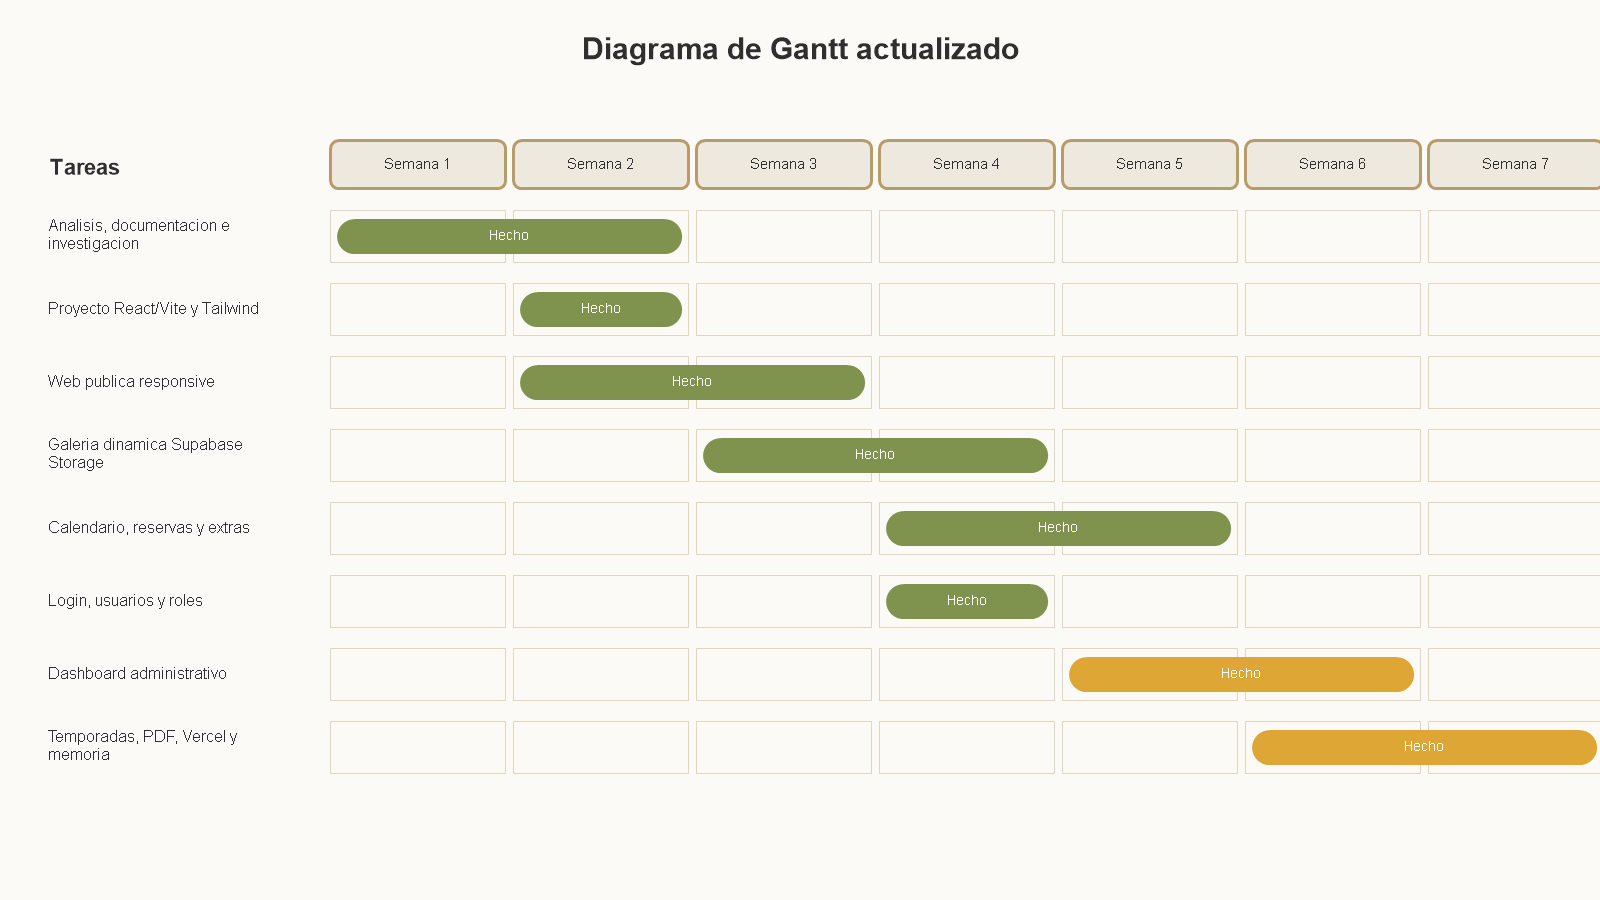
\includegraphics[width=\textwidth]{page-08-image-1.png}
  \caption{Diagrama de Gantt actualizado}
\end{figure}

\begin{table}[H]
\centering
\small
\begin{tabularx}{\textwidth}{|p{2cm}|p{4.9cm}|p{2.2cm}|X|}
\hline
\textbf{Fase} & \textbf{Plan inicial} & \textbf{Estado actual} & \textbf{Observación} \\
\hline
Fase 1 & Análisis, React, Supabase, casos de uso y modelo de datos. & Realizada & Se mantiene la base de análisis. \\
\hline
Fase 2 & Creación del proyecto, maquetación pública y conexión Supabase. & Realizada & La web pública está desarrollada y Supabase queda opcional. \\
\hline
Fase 3 & Disponibilidad, reserva, precios, calendario y bloqueos. & Avanzada & Calendario, guardado de reservas, cálculo de precios por temporada y extras están implementados; los bloqueos manuales quedan como mejora. \\
\hline
Fase 4 & Autenticación, roles, mis reservas, panel admin, temporadas y extras. & Avanzada & Autenticación, usuarios, panel administrativo, temporadas y extras están implementados; queda pendiente una vista específica de mis reservas para clientes. \\
\hline
Fase 5 & CSV/PDF, métricas, APIs externas, despliegue y documentación. & Parcial & Existe PDF de reserva, resumen administrativo y configuración de Vercel; quedan pendientes CSV e informes generales. \\
\hline
\end{tabularx}
\caption{Planificación actualizada}
\end{table}

\subsection{Secuencia de desarrollo del proyecto}
\begin{enumerate}[leftmargin=1.4cm]
  \item Creación del proyecto React/Vite.
  \item Investigación inicial de React, Vite y estructura de componentes.
  \item Configuración de Tailwind CSS y tema visual.
  \item Investigación de Tailwind CSS para sustituir estilos globales por clases de utilidad.
  \item Implementación de home con Hero, Info, Gallery, Reserva y Footer.
  \item Incorporación de fotografías reales y estructuras de datos de imágenes.
  \item Desarrollo de galería completa en la ruta \texttt{/galeria}.
  \item Investigación e implementación de calendario con \texttt{react-calendar} y lectura opcional desde Supabase.
  \item Implementación de formulario de reserva visual con selección de rango y cálculo de noches.
  \item Implementación de guardado real de reservas en Supabase.
  \item Incorporación de extras y cálculo de precios por temporadas.
  \item Implementación de login/registro con Supabase Auth y sincronización de usuarios.
  \item Investigación y migración de la galería a Supabase Storage con gestión dinámica por carpetas.
  \item Creación del dashboard administrativo y posterior refactor por secciones.
  \item Investigación de Recharts para representar métricas administrativas.
  \item Investigación e incorporación de generación de PDF para reservas con \texttt{jsPDF}.
  \item Configuración de despliegue en Vercel tras estudiar el funcionamiento de rutas SPA.
  \item Revisión de diferencias frente al documento anterior y actualización de la memoria.
\end{enumerate}

\subsection{Versionado de la aplicación: Git, ramas y pull requests}
El proyecto se ha gestionado con Git como sistema de control de versiones. Su uso ha sido fundamental para ordenar el desarrollo, conservar un historial de cambios y poder justificar la evolución real de la aplicación. Cada commit representa un avance concreto: creación inicial del proyecto, incorporación de componentes, integración de login, reservas, galería dinámica, dashboard y despliegue.

La rama principal del repositorio es \texttt{main}. Sobre ella se han ido integrando ramas funcionales mediante pull requests. Este enfoque permite trabajar una funcionalidad de forma aislada, probarla, revisar sus cambios y fusionarla posteriormente con la versión estable. En un proyecto que crece por módulos, esta separación reduce el riesgo de romper partes ya terminadas.

\subsubsection{Uso de commits}
Los commits se han utilizado como puntos de control del desarrollo. Algunos commits son pequeños y corrigen o ajustan una parte concreta, mientras que otros representan avances grandes, como la integración de reservas con Supabase o el refactor del dashboard por secciones. Esta trazabilidad permite reconstruir qué se hizo, cuándo se hizo y qué archivos se vieron afectados.

Ejemplos relevantes del historial:
\begin{itemize}[leftmargin=1.4cm]
  \item \texttt{71caca8}: primera versión del proyecto.
  \item \texttt{0b59c51}: integración de Tailwind CSS y refactor de estructura visual.
  \item \texttt{23fcf54}: integración de reservas con Supabase y extras.
  \item \texttt{b46bf0d}: gestión dinámica de galería con Supabase Storage.
  \item \texttt{b6de60b}: refactor del dashboard por secciones y corrección del alta de usuarios.
  \item \texttt{c72b77a}: configuración de despliegue en Vercel.
\end{itemize}

\subsubsection{Ramas funcionales}
Las ramas funcionales se han usado para separar bloques de trabajo. En lugar de desarrollar todo directamente sobre \texttt{main}, se crearon ramas orientadas a funcionalidades específicas. Esto facilita mantener el proyecto organizado y permite que cada módulo tenga su propio ciclo de desarrollo.

Las ramas más importantes han sido:
\begin{itemize}[leftmargin=1.4cm]
  \item \texttt{feature/login}: trabajo relacionado con autenticación, registro y acceso de usuarios.
  \item \texttt{feature/reservas}: integración de calendario, reservas, extras y persistencia en Supabase.
  \item \texttt{feature/dashboard}: creación y refactorización del panel administrativo.
\end{itemize}

\subsubsection{Pull requests e integración}
Los pull requests se han utilizado como puntos de integración entre ramas funcionales y \texttt{main}. Aunque el proyecto sea individual, usar pull requests aporta una forma profesional de cerrar fases de trabajo: se agrupan cambios, se revisa el alcance de la rama y se fusiona cuando el bloque está preparado.

\begin{table}[H]
\centering
\small
\begin{tabularx}{\textwidth}{|p{2.5cm}|p{3cm}|X|}
\hline
\textbf{Commit merge} & \textbf{Rama integrada} & \textbf{Funcionalidad asociada} \\
\hline
\texttt{a9d4e2d} & \texttt{feature/login} & Integración inicial del trabajo de login y autenticación. \\
\hline
\texttt{f1ba753} & \texttt{feature/reservas} & Integración del bloque de reservas, calendario y mejoras asociadas. \\
\hline
\texttt{9a2d0e3} & \texttt{feature/login} & Nueva integración de mejoras relacionadas con login e imágenes destacadas. \\
\hline
\texttt{872332b} & \texttt{feature/dashboard} & Integración del dashboard administrativo refactorizado por secciones. \\
\hline
\end{tabularx}
\caption{Pull requests e integraciones principales del repositorio}
\end{table}

\subsubsection{Ventajas aportadas al proyecto}
El versionado ha aportado varias ventajas prácticas:
\begin{itemize}[leftmargin=1.4cm]
  \item Permite documentar la evolución real del proyecto y relacionarla con la memoria.
  \item Facilita detectar desde qué commit aparece una funcionalidad.
  \item Ayuda a separar trabajo experimental de la rama principal.
  \item Permite integrar módulos completos, como reservas o dashboard, sin mezclar cambios inconexos.
  \item Sirve como apoyo al despliegue, ya que Vercel puede publicar una versión concreta del repositorio.
\end{itemize}

Por tanto, Git no se ha utilizado solo como copia de seguridad, sino como herramienta de organización, seguimiento, integración y despliegue del proyecto.

\subsection{Prototipo actualizado}
El PDF anterior describía el prototipo previsto. En esta segunda parte de la documentación se actualiza el prototipo según lo que ya existe en la aplicación:
\begin{itemize}[leftmargin=1.4cm]
  \item Página de inicio con información de La Galana, imagen principal y llamada a reservar.
  \item Galería destacada en la home mediante carrusel 3D.
  \item Página de galería completa con imágenes exteriores e interiores y visor ampliado.
  \item Sección de reserva con calendario visual y formulario de solicitud.
  \item Selección de extras durante el proceso de reserva.
  \item Accesos directos a Google Maps, llamada telefónica y WhatsApp.
  \item Página de login y registro con Supabase.
  \item Panel administrativo con resumen, reservas, galería y configuración.
  \item Gestión de imágenes de galería desde Supabase Storage.
  \item Generación de PDF asociado a una reserva.
\end{itemize}

Siguen pendientes dentro del prototipo completo: bloqueos manuales, validación avanzada de solapes, vista de mis reservas para clientes e informes CSV/PDF generales.

\section{Desarrollo del proyecto. ¿Qué se ha hecho realmente y cuánto tiempo se ha necesitado?}

\subsection{Secuencia real del desarrollo del proyecto}
\subsubsection{Variaciones respecto al plan inicial}
La comparación con el PDF anterior muestra estas variaciones principales:
\begin{itemize}[leftmargin=1.4cm]
  \item La galería completa y el carrusel 3D han avanzado más de lo previsto inicialmente.
  \item La autenticación ya existe, aunque en el PDF anterior aparecía como pendiente.
  \item La reserva como invitado se ha completado con persistencia real en Supabase, cálculo de precios y asociación de extras.
  \item La gestión de extras y temporadas se ha incorporado al dashboard de configuración.
  \item La galería ha pasado de usar imágenes locales a gestionarse dinámicamente con Supabase Storage.
  \item El panel administrativo se ha implementado y se ha refactorizado por secciones para mejorar su mantenimiento.
  \item La exportación PDF se ha incorporado para generar documentación de reservas.
  \item La validación avanzada de solapes, los bloqueos manuales y la vista de mis reservas siguen pendientes como mejoras futuras.
\end{itemize}

La secuencia real se ha desviado del plan inicial. Primero se consolidó la interfaz pública y, después, se añadieron los módulos de gestión interna: reservas reales, extras, temporadas, galería dinámica, usuarios, dashboard y PDF.

\begin{table}[H]
	\centering
	\small
	\renewcommand{\arraystretch}{1.25}
	\setlength{\tabcolsep}{4pt}
	
	\begin{tabularx}{\textwidth}{|p{2.7cm}|X|X|}
		\hline
		\textbf{Bloque desarrollado} & \textbf{Qué estaba escrito antes} & \textbf{Qué se ha hecho ahora} \\
		\hline
		
		Interfaz pública & Página principal con información. & Home completa con imagen principal, CTA de reserva, datos de la casa, galería destacada y footer. \\
		\hline
		
		Galería & Galería prevista. & Galería completa con categorías dinámicas, lightbox, navegación por teclado y carga desde Supabase Storage. \\
		\hline
		
		Calendario & Disponibilidad con reservas y bloqueos. & Consulta reservas reales de Supabase por mes activo y marca como ocupados los días incluidos entre entrada y salida. \\
		\hline
		
		Reserva & Reserva persistida como invitado. & Formulario con persistencia real, cálculo de noches, precios por temporada, extras y recarga del calendario. \\
		\hline
		
		Autenticación & Pendiente. & Login, registro, logout y sincronización de perfiles mediante Supabase Auth y tabla \texttt{usuarios}. \\
		\hline
		
		Panel administrativo & Previsto para una fase posterior. & Dashboard con resumen, reservas, galería y configuración para usuarios, extras y temporadas. \\
		\hline
		
		PDF & Exportaciones previstas. & Generación de documento PDF de reserva desde el panel administrativo con \texttt{jsPDF}. \\
		\hline
		
		Navegación & Header/footer básicos. & Navegación con rutas \texttt{/}, \texttt{/galeria}, \texttt{/login}, \texttt{/dashboard} y secciones internas del dashboard. \\
		\hline
		
	\end{tabularx}
	
	\caption{Variaciones respecto al plan inicial}
\end{table}

\subsection{Diagrama relacional, diagramas de clases y lógica de la aplicación}

\subsubsection{Modelo relacional}
\begin{figure}[H]
  \centering
  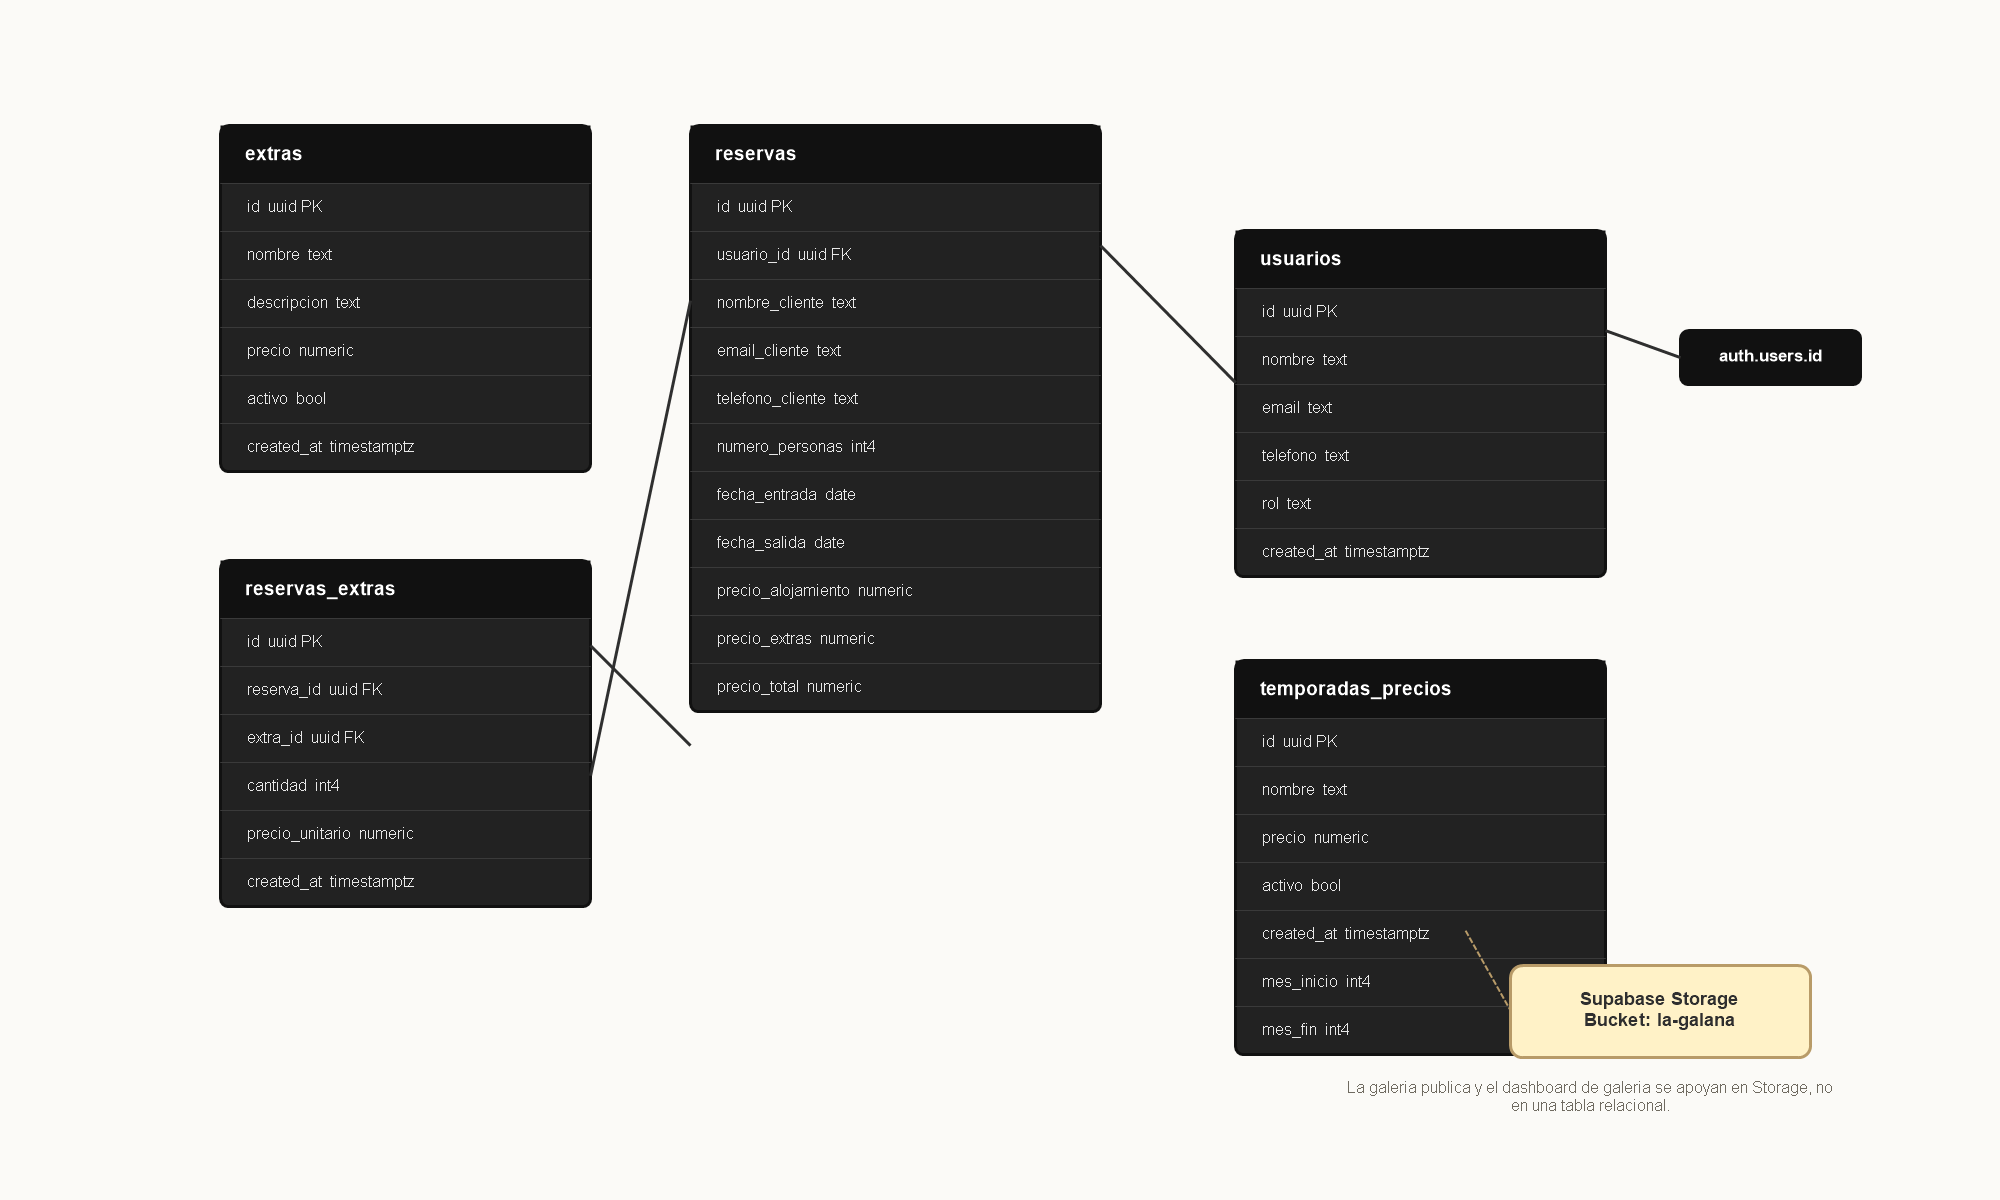
\includegraphics[width=\textwidth]{page-11-image-1.png}
  \caption{Diagrama relacional revisado}
\end{figure}

\subsubsection{Tablas de base de datos detalladas}
La base de datos actual se organiza en cinco tablas principales: \texttt{extras}, \texttt{reservas}, \texttt{reservas\_extras}, \texttt{temporadas\_precios} y \texttt{usuarios}. Este esquema sustituye el modelo anterior centrado en \texttt{clientes} y adapta la documentación al estado real del proyecto. Además, Supabase Storage se usa para almacenar las imágenes de la galería en el bucket público \texttt{la-galana}.

\paragraph{Extras}
\begin{table}[H]
\centering
\small
\begin{tabularx}{\textwidth}{|p{2.5cm}|p{2.2cm}|p{3.2cm}|X|}
\hline
\textbf{Campo} & \textbf{Tipo} & \textbf{Constraints} & \textbf{Descripción} \\
\hline
id & uuid & Primary & Identificador único del extra. \\
\hline
nombre & text & Unique & Nombre del extra. \\
\hline
descripcion & text & Nullable & Descripción opcional. \\
\hline
precio & numeric &  & Precio del extra. \\
\hline
activo & bool &  & Indica si el extra está disponible. \\
\hline
created\_at & timestamptz &  & Fecha de creación. \\
\hline
\end{tabularx}
\caption{Tabla de base de datos: extras}
\end{table}

\paragraph{Reservas}
\begin{table}[H]
\centering
\small
\begin{tabularx}{\textwidth}{|p{2.5cm}|p{2.2cm}|p{3.2cm}|X|}
\hline
\textbf{Campo} & \textbf{Tipo} & \textbf{Constraints} & \textbf{Descripción} \\
\hline
id & uuid & Primary & Identificador único de la reserva. \\
\hline
usuario\_id & uuid & Nullable & Usuario asociado a la reserva. \\
\hline
nombre\_cliente & text & Nullable & Nombre del cliente. \\
\hline
email\_cliente & text & Nullable & Correo electrónico del cliente. \\
\hline
telefono\_cliente & text & Nullable & Teléfono de contacto del cliente. \\
\hline
numero\_personas & int4 &  & Número de personas de la reserva. \\
\hline
created\_at & timestamptz &  & Fecha de creación. \\
\hline
fecha\_entrada & date & Nullable & Fecha de entrada. \\
\hline
fecha\_salida & date & Nullable & Fecha de salida. \\
\hline
precio\_alojamiento & numeric &  & Precio del alojamiento. \\
\hline
precio\_extras & numeric &  & Precio total de extras. \\
\hline
precio\_total & numeric &  & Precio total de la reserva. \\
\hline
\end{tabularx}
\caption{Tabla de base de datos: reservas}
\end{table}

\paragraph{Reservas extras}
\begin{table}[H]
\centering
\small
\begin{tabularx}{\textwidth}{|p{2.5cm}|p{2.2cm}|p{3.2cm}|X|}
\hline
\textbf{Campo} & \textbf{Tipo} & \textbf{Constraints} & \textbf{Descripción} \\
\hline
id & uuid & Primary & Identificador único del registro. \\
\hline
reserva\_id & uuid &  & Reserva asociada. \\
\hline
extra\_id & uuid &  & Extra asociado. \\
\hline
cantidad & int4 &  & Cantidad contratada. \\
\hline
precio\_unitario & numeric &  & Precio unitario aplicado. \\
\hline
created\_at & timestamptz &  & Fecha de creación. \\
\hline
\end{tabularx}
\caption{Tabla de base de datos: reservas\_extras}
\end{table}

\paragraph{Temporadas precios}
\begin{table}[H]
\centering
\small
\begin{tabularx}{\textwidth}{|p{2.5cm}|p{2.2cm}|p{3.2cm}|X|}
\hline
\textbf{Campo} & \textbf{Tipo} & \textbf{Constraints} & \textbf{Descripción} \\
\hline
id & uuid & Primary & Identificador único de la temporada. \\
\hline
nombre & text &  & Nombre de la temporada. \\
\hline
precio & numeric &  & Precio base. \\
\hline
activo & bool &  & Indica si la temporada está activa. \\
\hline
created\_at & timestamptz &  & Fecha de creación. \\
\hline
mes\_inicio & int4 &  & Mes de inicio. \\
\hline
mes\_fin & int4 &  & Mes de fin. \\
\hline
\end{tabularx}
\caption{Tabla de base de datos: temporadas\_precios}
\end{table}

\paragraph{Usuarios}
\begin{table}[H]
\centering
\small
\begin{tabularx}{\textwidth}{|p{2.5cm}|p{2.2cm}|p{3.2cm}|X|}
\hline
\textbf{Campo} & \textbf{Tipo} & \textbf{Constraints} & \textbf{Descripción} \\
\hline
id & uuid & Primary & Identificador único del usuario. \\
\hline
nombre & text &  & Nombre del usuario. \\
\hline
email & text & Unique & Correo electrónico del usuario. \\
\hline
telefono & text & Nullable & Teléfono de contacto. \\
\hline
rol & text &  & Rol del usuario. \\
\hline
created\_at & timestamptz &  & Fecha de creación. \\
\hline
\end{tabularx}
\caption{Tabla de base de datos: usuarios}
\end{table}

\begin{table}[H]
\centering
\small
\begin{tabularx}{\textwidth}{|p{3.2cm}|p{4.4cm}|X|}
\hline
\textbf{Entidad} & \textbf{Estado en el documento anterior} & \textbf{Estado en el código actual} \\
\hline
usuarios & No era el centro del modelo inicial. & Se usa para guardar perfiles de registro y consultar rol. \\
\hline
reservas & Tabla principal de reservas con estado y total. & Se usa para persistir solicitudes y calcular precios. \\
\hline
extras & No aparecía como tabla principal. & Tabla activa para extras contratables. \\
\hline
reservas\_extras & Tabla prevista. & Tabla activa para vincular extras con reservas. \\
\hline
temporadas\_precios & Entidad prevista para tarifas. & Tabla activa para definir precios y periodos. \\
\hline
storage.objects & No estaba contemplado en el modelo inicial. & Se usa para almacenar imágenes y carpetas de la galería dinámica. \\
\hline
\end{tabularx}
\caption{Modelo de datos revisado}
\end{table}

\paragraph{Supabase Storage y funciones RPC}
La galería se gestiona con un bucket público llamado \texttt{la-galana}. Cada carpeta del bucket funciona como categoría de galería y cada imagen se muestra en la web pública o en el dashboard administrativo. Para poder crear categorías vacías se utiliza un archivo marcador llamado \texttt{.emptyFolderPlaceholder}.

El fichero \texttt{supabase-galeria.sql} define las funciones necesarias para trabajar con Storage desde la aplicación:
\begin{itemize}[leftmargin=1.4cm]
  \item \texttt{es\_admin()}: comprueba si el usuario autenticado tiene rol de administrador.
  \item \texttt{crear\_categoria\_galeria(text)}: crea una carpeta/categoría en el bucket.
  \item \texttt{listar\_carpetas\_galeria()}: obtiene las categorías disponibles.
  \item \texttt{listar\_imagenes\_galeria(text)}: lista las imágenes de una categoría.
  \item \texttt{listar\_galeria\_storage()}: devuelve todas las imágenes agrupadas por carpeta.
\end{itemize}

También se definen políticas de acceso para permitir lectura pública de la galería y limitar la subida, edición o borrado de imágenes a usuarios administradores. Además, se crea un trigger sobre \texttt{auth.users} para sincronizar los nuevos registros con la tabla pública \texttt{usuarios}.

\subsubsection{Estructura de clases/componentes actual}
\begin{figure}[H]
  \centering
  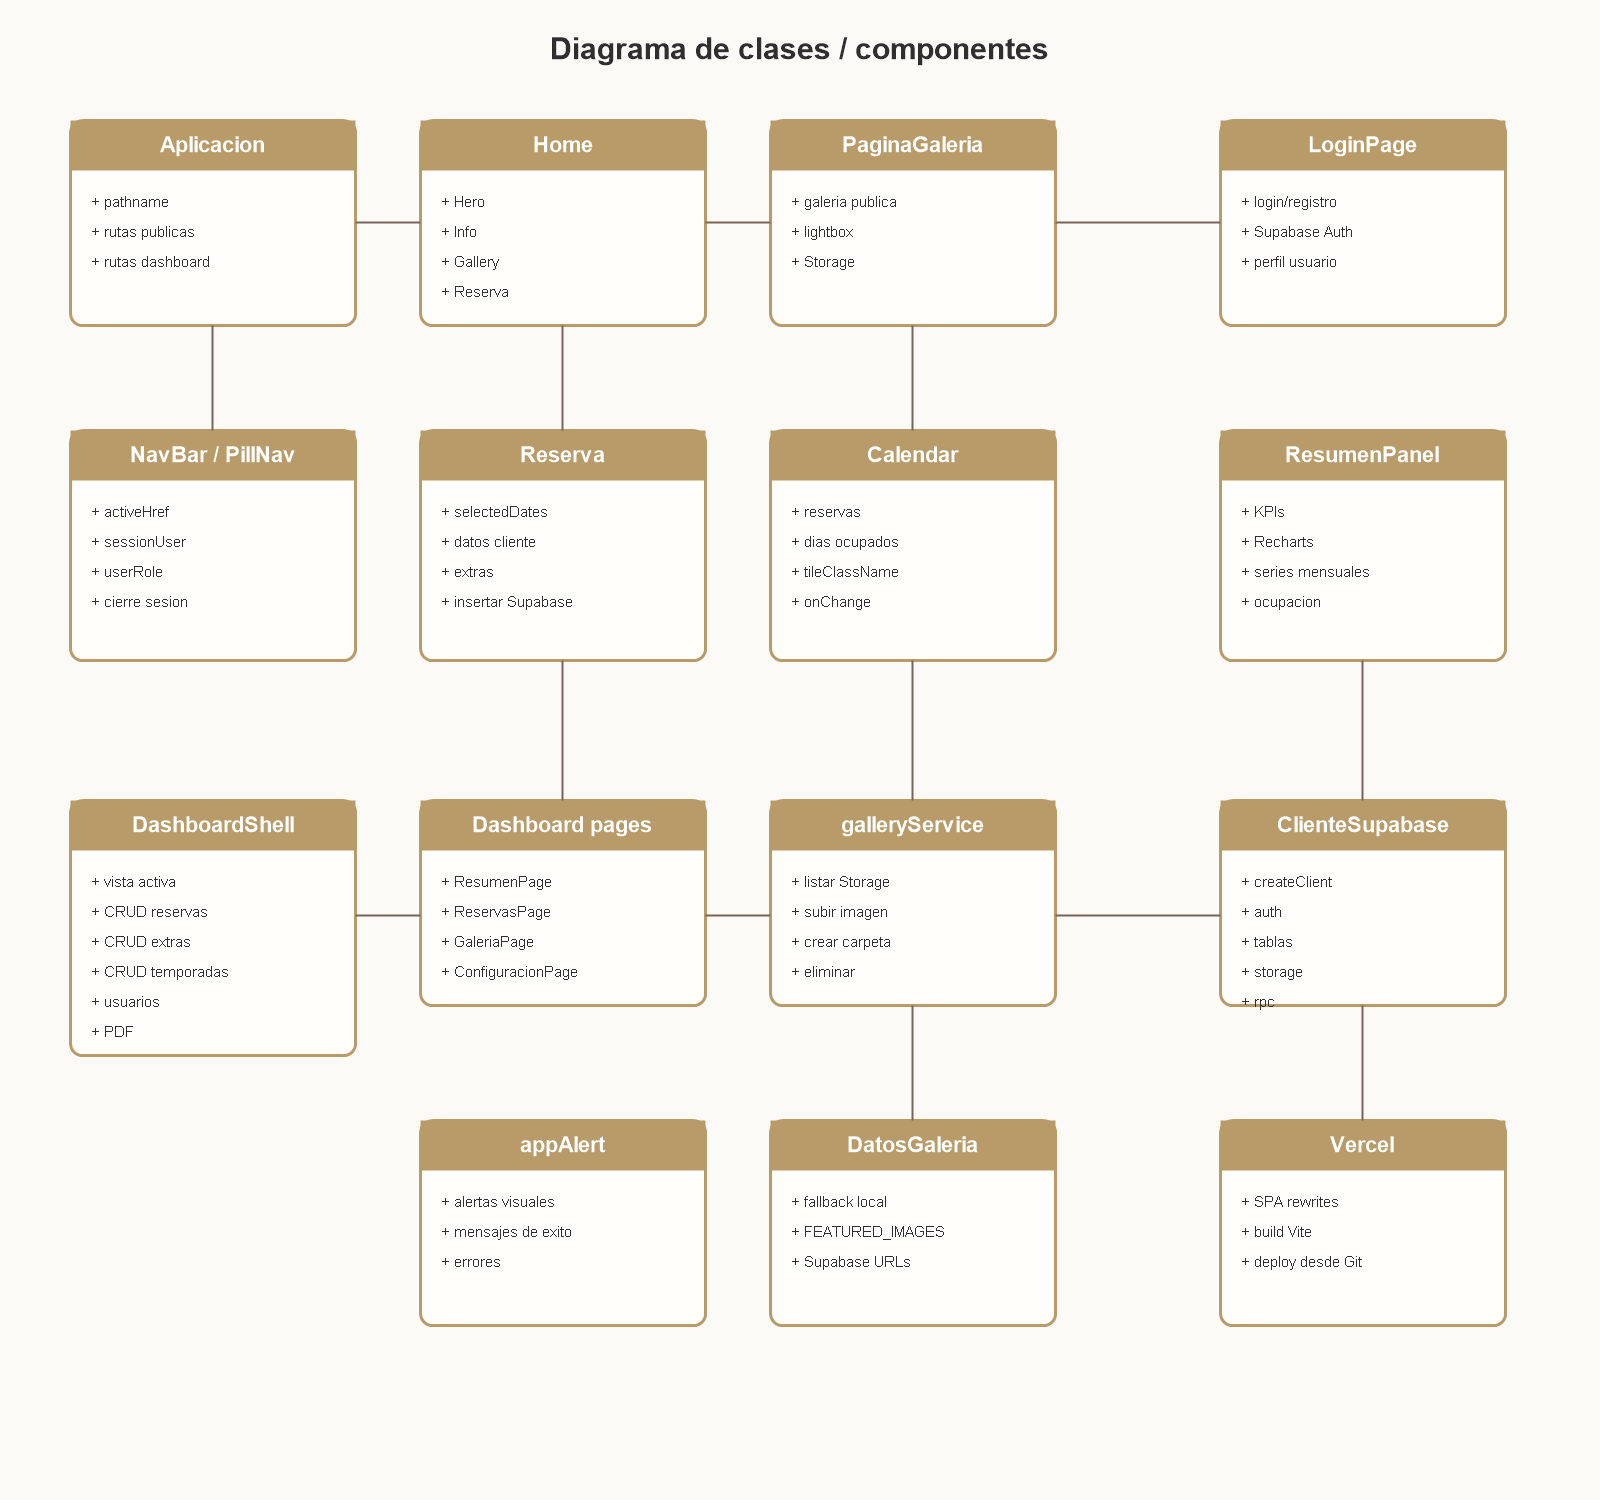
\includegraphics[width=\textwidth]{page-12-image-1.png}
  \caption{Diagrama de clases / componentes con nombres reales en español}
\end{figure}

\begin{table}[H]
\centering
\small
\begin{tabularx}{\textwidth}{|p{6.0cm}|X|}
\hline
\textbf{Fichero} & \textbf{Responsabilidad} \\
\hline
\texttt{src/App.jsx} & Control de vistas según pathname: \texttt{/}, \texttt{/galeria}, \texttt{/login} y rutas del dashboard. \\
\hline
\texttt{src/pages/Home.jsx} & Composición de la página principal. \\
\hline
\texttt{src/pages/GalleryPage.jsx} & Galería completa, secciones, lightbox y navegación. \\
\hline
\texttt{src/pages/LoginPage.jsx} & Login, registro, cierre de sesión y sincronización de perfil con Supabase. \\
\hline
\texttt{src/components/NavBar.jsx} & Navegación, sesión activa, rol y logout. \\
\hline
\texttt{src/components/Calendar.jsx} & Calendario, lectura de reservas y clases de estado. \\
\hline
\texttt{src/components/Reserva.jsx} & Formulario, selección de fechas, extras, cálculo de precios y guardado de reservas. \\
\hline
\texttt{src/components/ThreeDCarousel.jsx} & Carrusel interactivo con rotación y controles. \\
\hline
\texttt{src/components/ResumenPanel.jsx} & Tarjetas e indicadores de resumen usados en el panel administrativo. \\
\hline
\texttt{src/pages/dashboard/DashboardShell.jsx} & Estructura principal del dashboard y operaciones de gestión. \\
\hline
\texttt{src/pages/dashboard/ResumenPage.jsx} & Entrada a la vista de resumen del dashboard. \\
\hline
\texttt{src/pages/dashboard/ReservasPage.jsx} & Entrada a la gestión de reservas. \\
\hline
\texttt{src/pages/dashboard/GaleriaPage.jsx} & Entrada a la gestión de galería. \\
\hline
\texttt{src/pages/dashboard/ConfiguracionPage.jsx} & Entrada a configuración de usuarios, extras y temporadas. \\
\hline
\texttt{src/pages/dashboard/useDatosDashboard.js} & Hook para cargar reservas, usuarios, extras, temporadas y galería. \\
\hline
\texttt{src/services/galleryService.js} & Servicio de lectura, subida y borrado de imágenes en Supabase Storage. \\
\hline
\texttt{src/data/laGalanaImages.js} & Imágenes destacadas y datos de apoyo para la web pública. \\
\hline
\texttt{src/supabase/client.js} & Cliente Supabase opcional según variables de entorno. \\
\hline
\texttt{supabase-galeria.sql} & Configuración SQL de Storage, funciones RPC, trigger de usuarios y políticas de seguridad. \\
\hline
\texttt{vercel.json} & Configuración de despliegue SPA en Vercel. \\
\hline
\end{tabularx}
\caption{Estructura de clases/componentes actual}
\end{table}

\subsubsection{Lógica actual de la aplicación}
\begin{itemize}[leftmargin=1.4cm]
  \item La navegación se controla con pathname y un evento personalizado \texttt{app:navigate}.
  \item El calendario consulta reservas de Supabase si existen \texttt{VITE\_SUPABASE\_URL} y \texttt{VITE\_SUPABASE\_ANON\_KEY}.
  \item Cada día del calendario se pinta como disponible u ocupado según las fechas de entrada y salida de las reservas.
  \item El formulario de reserva valida los datos principales, calcula noches, consulta temporadas, suma extras y guarda la reserva en Supabase.
  \item Si hay extras seleccionados, se insertan registros en \texttt{reservas\_extras} con cantidad y precio unitario.
  \item El login usa Supabase Auth y sincroniza los datos de perfil en la tabla \texttt{usuarios}.
  \item El dashboard carga en paralelo reservas, usuarios, extras, temporadas y galería mediante \texttt{useDatosDashboard}.
  \item La galería se obtiene desde Supabase Storage mediante funciones RPC y URLs públicas.
  \item El panel administrativo permite crear, editar y eliminar reservas, usuarios, extras, temporadas e imágenes.
  \item La generación PDF crea una ficha de reserva y formularios de viajero con \texttt{jsPDF}.
\end{itemize}

\subsection{Interacción con el usuario}

\subsubsection{Casos de uso / historias de usuario}
Además de los diagramas, se describen los casos de uso heredados del PDF anterior y se actualiza su estado:

\begin{table}[H]
	\centering
	\small
	\renewcommand{\arraystretch}{1.25}
	\setlength{\tabcolsep}{4pt}
	
	\begin{tabularx}{\textwidth}{|p{2.8cm}|X|X|	}
		\hline
		\textbf{Caso de uso} & \textbf{Descripción} & \textbf{Estado en la aplicación actual} \\
		\hline
		
		Consultar disponibilidad & El usuario revisa el calendario para ver fechas disponibles u ocupadas. & Implementado con lectura de reservas en Supabase. \\
		\hline
		
		Reservar como invitado & El usuario introduce datos personales, selecciona fechas y puede añadir extras. & Implementado con guardado en Supabase. \\
		\hline
		
		Registro/Login de cliente & El usuario crea cuenta o inicia sesión. & Implementado con Supabase Auth y perfil en tabla \texttt{usuarios}. \\
		\hline
		
		Administrar reservas & Crear, editar, eliminar y generar PDF de reservas. & Implementado en el dashboard. \\
		\hline
		
		Gestionar temporadas y extras & Configurar precios por periodo y servicios adicionales. & Implementado en configuración del dashboard. \\
		\hline
		
		Gestionar galería & Crear categorías, subir imágenes y eliminar elementos. & Implementado con Supabase Storage. \\
\hline
		
		Gestionar usuarios & Consultar, filtrar, crear, editar o eliminar usuarios. & Implementado en configuración del dashboard. \\
\hline
		
		Exportaciones & Generar CSV y PDF. & PDF implementado para reservas; CSV queda como ampliación. \\
		\hline
		
	\end{tabularx}
	
	\caption{Casos de uso actualizados}
\end{table}

\begin{figure}[H]
  \centering
  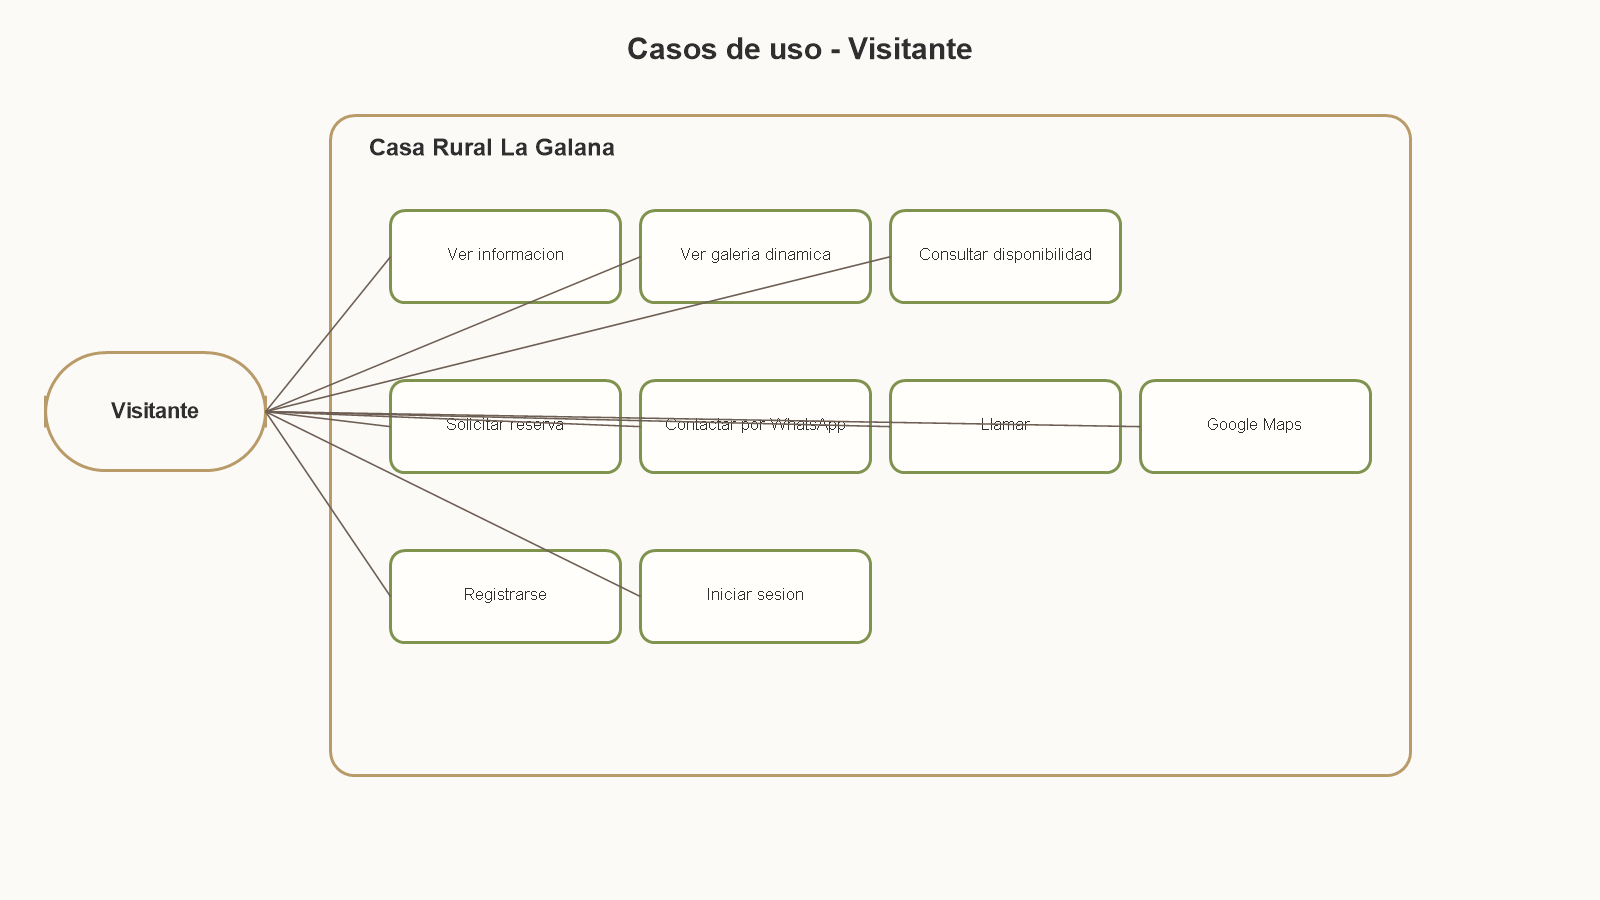
\includegraphics[width=\textwidth]{page-14-image-1.png}
  \caption{Casos de uso del Visitante}
\end{figure}

\begin{figure}[H]
  \centering
  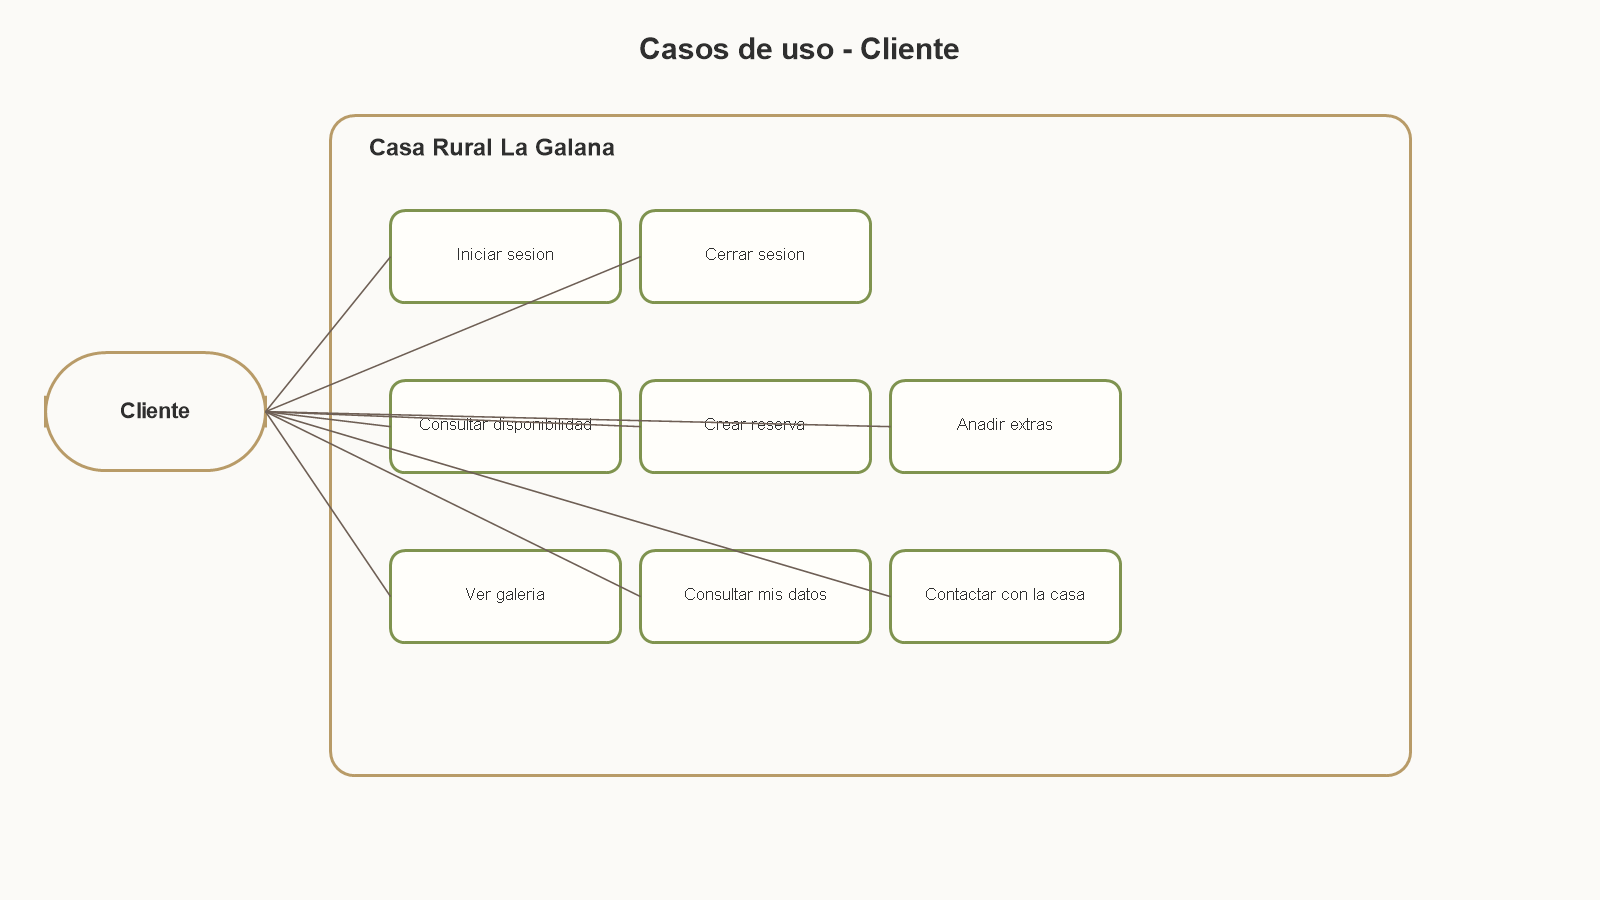
\includegraphics[width=\textwidth]{page-14-image-2.png}
  \caption{Casos de uso del Cliente}
\end{figure}

\begin{figure}[H]
  \centering
  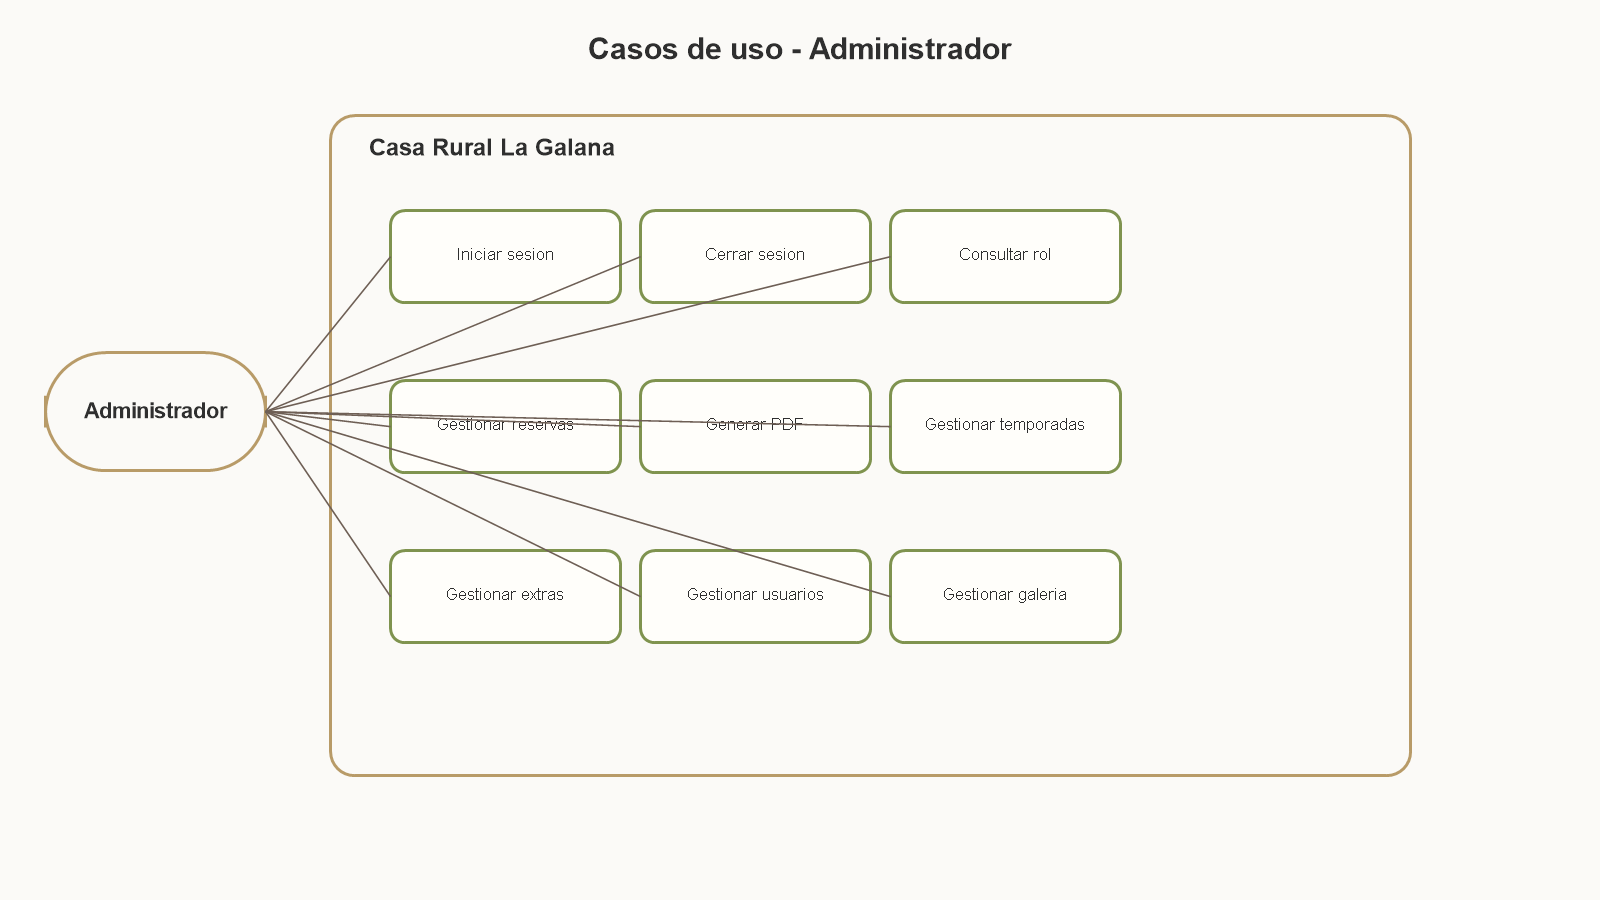
\includegraphics[width=\textwidth]{page-15-image-1.png}
  \caption{Casos de uso del Administrador}
\end{figure}

\begin{figure}[H]
  \centering
  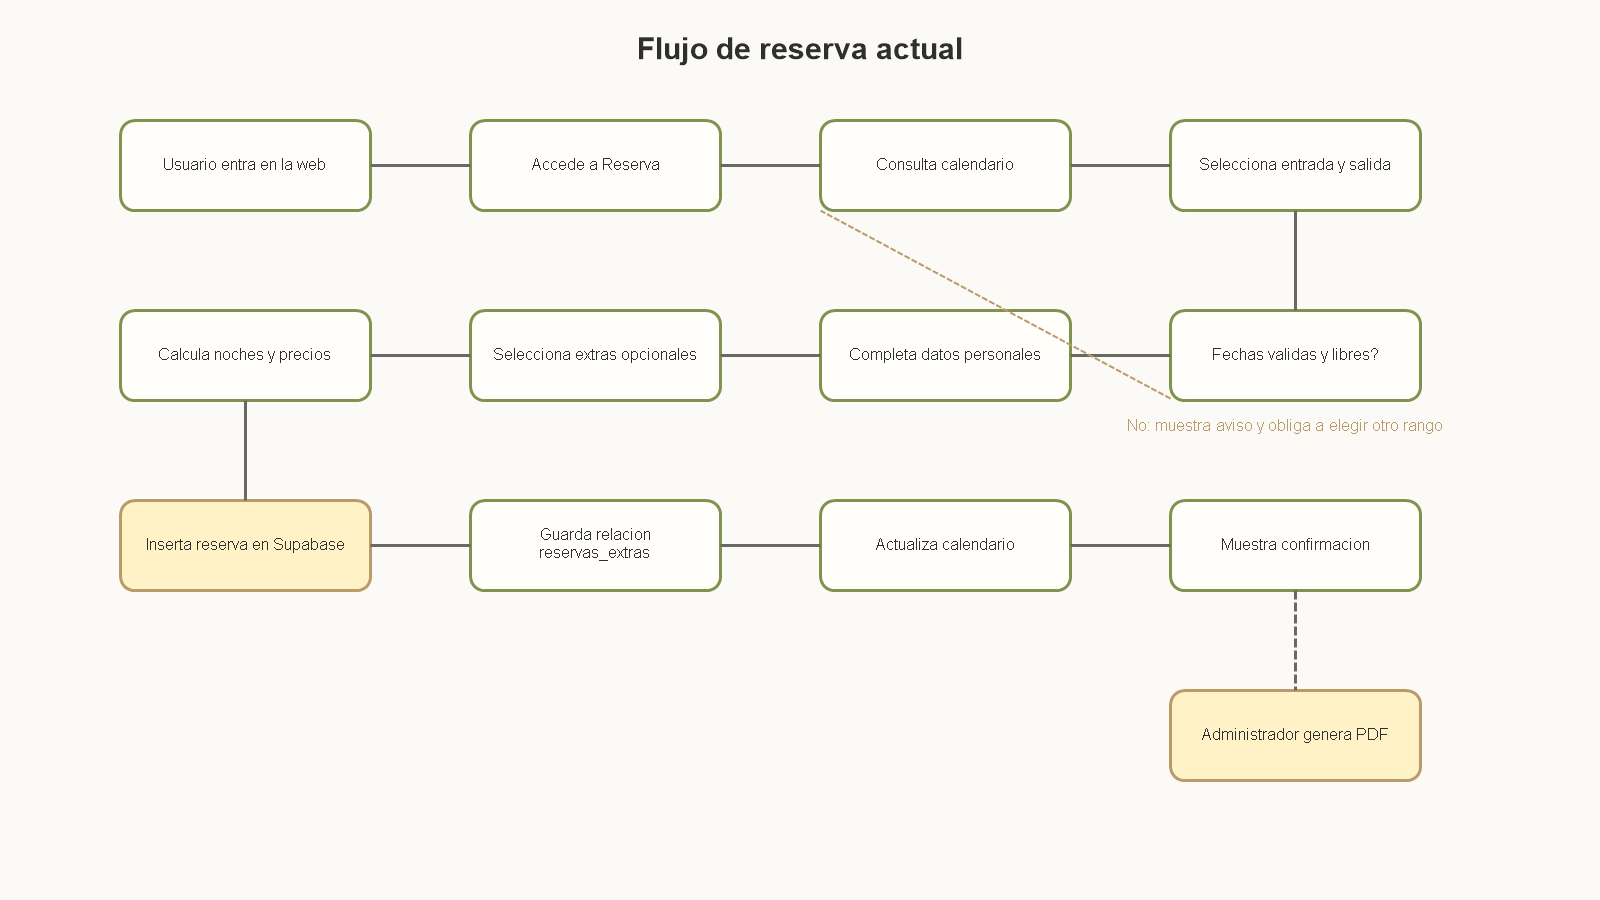
\includegraphics[width=\textwidth]{page-16-image-1.png}
  \caption{Diagrama de flujo de reserva actual}
\end{figure}

\begin{table}[H]
\centering
\small
\begin{tabularx}{\textwidth}{|p{4.6cm}|p{2.4cm}|X|}
\hline
\textbf{Caso de uso} & \textbf{Estado actual} & \textbf{Descripción} \\
\hline
Consultar información de la casa & Implementado & El usuario accede a la home y consulta capacidad y características. \\
\hline
Ver galería completa & Implementado & El usuario accede a \texttt{/galeria}, revisa imágenes y usa lightbox. \\
\hline
Consultar disponibilidad & Implementado & El usuario ve calendario con ocupación calculada desde reservas guardadas en Supabase. \\
\hline
Solicitar reserva & Implementado & El usuario selecciona fechas, completa datos, añade extras y la reserva se guarda en Supabase. \\
\hline
Registrarse & Implementado con Supabase & Crea cuenta y perfil con rol cliente si hay configuración. \\
\hline
Iniciar sesión & Implementado & Acceso con Supabase Auth. \\
\hline
Administrar reservas & Implementado & El administrador consulta, crea, edita, elimina y genera PDF de reservas. \\
\hline
Gestionar galería & Implementado & El administrador crea categorías, sube imágenes y elimina recursos del bucket. \\
\hline
Gestionar extras y temporadas & Implementado & El administrador mantiene servicios adicionales y precios por periodo. \\
\hline
Gestionar usuarios & Implementado & El administrador consulta, filtra y mantiene perfiles de usuario. \\
\hline
Exportar informes & Parcial & Existe PDF de reserva; quedan pendientes CSV e informes generales. \\
\hline
\end{tabularx}
\caption{Desglose funcional de casos de uso}
\end{table}

\subsection{Diseño de la interfaz}
La interfaz pública utiliza una estética cálida y rural. Se combinan tonos beige, verde y gris oscuro con fotografías reales. La fuente Playfair Display se usa para títulos y la fuente Inter para contenido. La web está pensada para uso responsive y prioriza la imagen del alojamiento.

El panel administrativo utiliza un diseño más funcional, basado en tarjetas, tablas, métricas, filtros y modales de edición. La navegación se divide por secciones para separar el resumen general, la gestión de reservas, la administración de galería y la configuración de usuarios, extras y temporadas. Esta diferencia de enfoque permite que la parte pública sea visual y comercial, mientras que el dashboard prioriza claridad, rapidez de consulta y mantenimiento de datos.

\subsection{Código fuente}
En este apartado se recogen fragmentos reales del código de la aplicación. Se han seleccionado partes representativas de cada tecnología principal para mostrar no solo que se han usado, sino cómo se integran internamente dentro del proyecto.

\subsubsection{React: control de rutas y composición de páginas}
El componente principal \texttt{App.jsx} controla la vista actual leyendo el \texttt{pathname}. En lugar de usar un router externo, la aplicación escucha cambios de historial y un evento personalizado llamado \texttt{app:navigate}. Esto permite cambiar entre la web pública, la galería, el login y el dashboard.

\begin{verbatim}
function Aplicacion() {
  const [pathname, setPathname] = useState(window.location.pathname);

  useEffect(() => {
    const manejarCambioRuta = () => setPathname(window.location.pathname);

    window.addEventListener("popstate", manejarCambioRuta);
    window.addEventListener("app:navigate", manejarCambioRuta);

    return () => {
      window.removeEventListener("popstate", manejarCambioRuta);
      window.removeEventListener("app:navigate", manejarCambioRuta);
    };
  }, []);

  if (pathname === "/galeria") return <PaginaGaleria />;
  if (pathname === "/login") return <PaginaLogin />;
  if (pathname === "/dashboard" || pathname === "/dashboard/resumen") {
    return <PaginaResumenDashboard />;
  }
  if (pathname === "/dashboard/reservas") return <PaginaReservasDashboard />;
  if (pathname === "/dashboard/galeria") return <PaginaGaleriaDashboard />;
  if (pathname === "/dashboard/configuracion") {
    return <PaginaConfiguracionDashboard />;
  }

  return <Inicio />;
}
\end{verbatim}

\subsubsection{Supabase: inicialización segura del cliente}
El cliente de Supabase se inicializa solo si existen las variables de entorno necesarias. Esta decisión evita que la aplicación quede en blanco cuando se ejecuta sin configuración de backend, algo importante durante desarrollo, pruebas o despliegues incompletos.

\begin{verbatim}
import { createClient } from "@supabase/supabase-js";

const url = import.meta.env.VITE_SUPABASE_URL;
const key = import.meta.env.VITE_SUPABASE_ANON_KEY;

export const supabase =
  url && key ? createClient(url, key) : null;

if (import.meta.env.DEV && supabase) {
  window.supabase = supabase;
}
\end{verbatim}

\subsubsection{Reservas: cálculo de precios, extras y persistencia}
El formulario de reserva no se limita a recoger datos. Antes de guardar, calcula las noches, consulta las temporadas activas, suma los extras seleccionados y persiste tanto la reserva principal como la relación con \texttt{reservas\_extras}.

\begin{verbatim}
const precioAlojamiento = await calcularPrecioAlojamiento(
  selectedDates[0],
  selectedDates[1],
);
const precioExtras = extrasSeleccionados.reduce(
  (total, extra) => total + extra.precio * extra.cantidad,
  0,
);
const precioTotal = precioAlojamiento + precioExtras;

const { data: reservaGuardada, error: errorReserva } = await supabase
  .from("reservas")
  .insert({
    usuario_id: user?.id ?? null,
    nombre_cliente: reservationData.name,
    email_cliente: reservationData.email,
    telefono_cliente: reservationData.phone || null,
    fecha_entrada: formatearFechaSql(selectedDates[0]),
    fecha_salida: formatearFechaSql(selectedDates[1]),
    numero_personas: Number(reservationData.guests),
    precio_alojamiento: precioAlojamiento,
    precio_extras: precioExtras,
    precio_total: precioTotal,
  })
  .select("id")
  .single();

if (extrasSeleccionados.length > 0) {
  const reservasExtras = extrasSeleccionados.map((extra) => ({
    reserva_id: reservaGuardada.id,
    extra_id: extra.id,
    cantidad: extra.cantidad,
    precio_unitario: extra.precio,
  }));

  await supabase.from("reservas_extras").insert(reservasExtras);
}
\end{verbatim}

\subsubsection{React Calendar: disponibilidad y estados visuales}
El calendario obtiene las reservas de Supabase y convierte cada rango de entrada/salida en un conjunto de días ocupados. Después, cada celda del calendario puede clasificarse como disponible u ocupada.

\begin{verbatim}
const diasReservados = useMemo(() => {
  const fechas = new Set();

  reservas.forEach((reserva) => {
    const fechaEntrada = crearFechaDesdeSql(reserva.fecha_entrada);
    const fechaSalida = crearFechaDesdeSql(reserva.fecha_salida);
    if (!fechaEntrada || !fechaSalida) return;

    const fechaActual = new Date(fechaEntrada);
    while (fechaActual <= fechaSalida) {
      fechas.add(formatearFecha(fechaActual));
      fechaActual.setDate(fechaActual.getDate() + 1);
    }
  });

  return fechas;
}, [reservas]);

const { data, error } = await supabase
  .from("reservas")
  .select("fecha_entrada, fecha_salida")
  .lte("fecha_entrada", formatearFecha(ultimoDia))
  .gte("fecha_salida", formatearFecha(primerDia));

const obtenerEstado = (date) => {
  return diasReservados.has(formatearFecha(date))
    ? "confirmada"
    : "disponible";
};
\end{verbatim}

\subsubsection{Tailwind CSS: personalización visual del calendario}
Tailwind se usa tanto en el JSX como en el CSS global. En el calendario se combinan clases de la librería \texttt{react-calendar} con utilidades Tailwind mediante \texttt{@apply}, lo que permite adaptar un componente externo al estilo propio de La Galana.

\begin{verbatim}
.calendar-shell .react-calendar {
  @apply w-full max-w-none rounded-[1.7rem] border border-white/14
  bg-white/10 p-3 text-white shadow-none backdrop-blur-md sm:p-4 lg:p-5;
}

.calendar-shell .react-calendar__tile {
  @apply relative min-h-[56px] rounded-2xl border border-transparent
  bg-transparent px-1 py-3 text-sm font-semibold text-white transition
  sm:min-h-[68px] sm:py-4;
}

.calendar-shell .react-calendar__tile.disponible {
  @apply border-accent/20 bg-accent/18;
}

.calendar-shell .react-calendar__tile.confirmada {
  @apply border-red-700/25 bg-red-700;
}
\end{verbatim}

\subsubsection{Supabase Storage: galería dinámica}
La galería ya no depende solo de imágenes locales. El servicio \texttt{galleryService.js} consulta carpetas e imágenes desde Supabase Storage mediante funciones RPC y construye categorías que después se muestran en la web pública y en el dashboard.

\begin{verbatim}
async function listarCarpetasAlmacenamiento() {
  const { data, error } = await supabase.rpc("listar_carpetas_galeria");
  if (error) return { folders: [], error };

  const folders = [...new Set((data || [])
    .map((item) => item.carpeta)
    .filter(Boolean))]
    .sort();

  return { folders, error: null };
}

async function listarTodasLasImagenesGaleria() {
  const { data, error } = await supabase.rpc("listar_galeria_storage");
  return { rows: data || [], error };
}

export async function subirImagenGaleria({ category, file, title }) {
  const finalName = title ? `${Date.now()}-${safeTitle}${extension}` : safeName;
  const storagePath = `${category.slug}/${finalName}`;

  return supabase.storage.from("la-galana").upload(storagePath, file, {
    cacheControl: "3600",
    upsert: false,
    contentType: file.type || "image/webp",
  });
}
\end{verbatim}

\subsubsection{Recharts: métricas del dashboard}
Recharts recibe datos ya transformados. Primero se agrupan los registros por mes y después se renderiza una gráfica de líneas con ejes, tooltip y leyenda. Esto permite convertir las reservas en información visual para el administrador.

\begin{verbatim}
function crearSerieMensual({ registros, selector, meses }) {
  const mapa = new Map(meses.map((mes) => [claveMes(mes.fecha), 0]));

  registros.forEach((registro) => {
    const fechaReferencia =
      crearFechaDesdeSql(registro.created_at) ||
      crearFechaDesdeSql(registro.fecha_entrada);
    if (!fechaReferencia) return;

    const clave = claveMes(fechaReferencia);
    if (!mapa.has(clave)) return;

    mapa.set(clave, mapa.get(clave) + Number(selector(registro) || 0));
  });

  return meses.map((mes) => mapa.get(claveMes(mes.fecha)) || 0);
}

<ResponsiveContainer width="100%" height="100%">
  <LineChart data={datos}>
    <XAxis dataKey="etiqueta" />
    <YAxis tickFormatter={formatearEtiqueta} />
    <Tooltip formatter={(value) => [formatearValor(Number(value)), ""]} />
    <Legend />
    {series.map((serie) => (
      <Line
        key={serie.label}
        type="monotone"
        dataKey={serie.label}
        stroke={serie.color}
        strokeWidth={3}
      />
    ))}
  </LineChart>
</ResponsiveContainer>
\end{verbatim}

\subsubsection{jsPDF: generación de documentos de reserva}
El dashboard puede generar un documento PDF a partir de una reserva. El código crea un A4, escribe los datos principales y añade páginas para viajeros según el número de personas de la reserva.

\begin{verbatim}
function generarPdfReserva(reserva) {
  if (!reserva) return;

  const doc = new jsPDF({ unit: "mm", format: "a4" });
  const numeroPersonas = Math.max(1, Number(reserva.numero_personas || 1));

  dibujarCabeceraPdf(doc, "Datos de la reserva", "Casa Rural La Galana", 1);

  doc.setFont("helvetica", "bold");
  doc.setFontSize(14);
  doc.text("Resumen de la reserva", 14, 32);

  const datosReserva = [
    ["Cliente", reserva.nombre_cliente],
    ["Email", reserva.email_cliente],
    ["Entrada", obtenerFechaLegible(reserva.fecha_entrada)],
    ["Salida", obtenerFechaLegible(reserva.fecha_salida)],
    ["Total", formatearMoneda(reserva.precio_total)],
  ];

  datosReserva.forEach(([etiqueta, valor], index) => {
    const columnaX = index % 2 === 0 ? 14 : 108;
    dibujarLineaCampo(doc, etiqueta, valor, columnaX, y, 78);
  });

  for (let viajero = 1; viajero <= numeroPersonas; viajero += 1) {
    doc.addPage();
    dibujarCabeceraPdf(doc, "Formulario de viajero", "Reserva", viajero + 1);
  }
}
\end{verbatim}

\subsubsection{Vercel: configuración de rutas SPA}
El despliegue en Vercel necesita una configuración específica para que las rutas internas de React funcionen al recargar la página. La regla siguiente indica que cualquier ruta debe devolver \texttt{index.html}.

\begin{verbatim}
{
  "rewrites": [
    {
      "source": "/(.*)",
      "destination": "/index.html"
    }
  ]
}
\end{verbatim}

\section{Fase de pruebas}

\subsection{Pruebas realizadas}
Las pruebas se han planteado como una validación funcional por módulos. La aplicación no dispone todavía de una batería automatizada, por lo que la comprobación se ha realizado mediante casos manuales que reproducen el comportamiento esperado de un usuario real y de un administrador. Para cada caso se indica el objetivo, los datos de entrada, los pasos y el resultado esperado.

El criterio utilizado para considerar una prueba correcta ha sido doble: por un lado, que la interfaz responda sin errores visibles; por otro, que el cambio quede reflejado en Supabase cuando la prueba modifica datos persistentes. En los casos relacionados con galería, reservas, extras o temporadas, la validación no se limita a pulsar botones, sino que también comprueba que la información almacenada es coherente con lo mostrado por la aplicación.

\begin{table}[H]
\centering
\small
\begin{tabularx}{\textwidth}{|p{2.8cm}|p{2.7cm}|p{3.2cm}|p{2.9cm}|p{3.1cm}|}
\hline
\textbf{Caso de prueba} & \textbf{Objetivo} & \textbf{Datos de entrada} & \textbf{Pasos a seguir} & \textbf{Resultado esperado} \\
\hline
Consulta disponibilidad & Verificar calendario & Mes cualquiera & 1. Entrar en Reserva. 2. Cambiar de mes. 3. Observar colores. & Se muestran fechas disponibles u ocupadas según reservas reales. \\
\hline
Selección de rango & Validar selección de entrada y salida & Dos fechas & 1. Seleccionar inicio. 2. Seleccionar fin. & Se muestra el rango seleccionado y número de noches. \\
\hline
Reserva sin fechas & Comprobar validación & Formulario sin rango completo & 1. Rellenar datos. 2. Enviar sin fechas. & Aparece alerta solicitando seleccionar fechas. \\
\hline
Solicitud de reserva & Comprobar persistencia & Nombre, email, teléfono, fechas y personas & 1. Rellenar formulario. 2. Enviar. 3. Consultar Supabase. & La reserva se guarda, aparece alerta de éxito y se limpia el formulario. \\
\hline
Reserva con extras & Comprobar relación con extras & Fechas y extras seleccionados & 1. Abrir modal de extras. 2. Seleccionar servicios. 3. Enviar reserva. & Se guardan la reserva y sus registros en \texttt{reservas\_extras}. \\
\hline
Precio por temporada & Verificar cálculo de importe & Fechas en una temporada activa & 1. Configurar temporada. 2. Crear reserva. & El precio del alojamiento se calcula con la tarifa correspondiente. \\
\hline
Login Supabase & Validar acceso real & Email y contraseña válidos & 1. Entrar en Login. 2. Introducir credenciales. & Se inicia sesión y se actualiza la navegación. \\
\hline
Registro Supabase & Validar registro real & Nombre, email y contraseña & 1. Configurar Supabase. 2. Crear cuenta. & Se crea usuario y perfil con rol cliente. \\
\hline
Dashboard reservas & Verificar gestión administrativa & Reserva existente & 1. Entrar en \texttt{/dashboard/reservas}. 2. Editar una reserva. 3. Guardar. & La reserva se actualiza en Supabase. \\
\hline
PDF de reserva & Verificar generación documental & Reserva existente & 1. Entrar en dashboard. 2. Pulsar PDF. & Se abre/genera un documento PDF con datos de la reserva. \\
\hline
Gestión de galería & Verificar Storage & Imagen y categoría & 1. Crear categoría. 2. Subir imagen. 3. Revisar galería. & La imagen queda disponible mediante Supabase Storage. \\
\hline
Gestión de configuración & Verificar extras y temporadas & Datos de extra o temporada & 1. Crear o editar registro. 2. Guardar. & El registro se actualiza y queda disponible para reservas. \\
\hline
Navegación & Verificar rutas principales & Usuario en la app & 1. Ir a Inicio. 2. Ir a Galería. 3. Ir a Login. 4. Ir a Dashboard. & Todas las vistas cargan sin errores. \\
\hline
\end{tabularx}
\caption{Batería de pruebas funcionales principales}
\end{table}

\begin{table}[H]
\centering
\small
\begin{tabularx}{\textwidth}{|p{2.8cm}|p{2.7cm}|p{3.2cm}|p{2.9cm}|p{3.1cm}|}
\hline
\textbf{Caso de prueba} & \textbf{Objetivo} & \textbf{Datos de entrada} & \textbf{Pasos a seguir} & \textbf{Resultado esperado} \\
\hline
Acceso administrativo & Validar rutas privadas a nivel funcional & Usuario administrador & 1. Iniciar sesión. 2. Entrar en Dashboard. 3. Navegar por secciones. & El administrador puede acceder al panel y ver las opciones de gestión. \\
\hline
Acceso cliente & Comprobar experiencia de usuario no administrador & Usuario cliente & 1. Iniciar sesión como cliente. 2. Usar navegación principal. & El usuario conserva una experiencia orientada a reserva y consulta, sin etiqueta de empleado. \\
\hline
Eliminación de registros & Verificar borrado controlado & Reserva, extra o imagen existente & 1. Seleccionar registro. 2. Pulsar eliminar. 3. Confirmar acción. & El elemento desaparece de la vista y se elimina de Supabase o Storage. \\
\hline
Actualización de métricas & Comprobar dashboard & Reservas existentes & 1. Crear o modificar una reserva. 2. Volver a resumen. & Las tarjetas y gráficos reflejan los datos actualizados. \\
\hline
Rutas en producción & Validar comportamiento SPA & Ruta directa de dashboard o galería & 1. Abrir ruta directamente. 2. Recargar navegador. & Vercel redirige correctamente a la aplicación sin error 404. \\
\hline
\end{tabularx}
\caption{Batería de pruebas complementarias}
\end{table}

\subsubsection{Pruebas pendientes de automatizar}
No se han localizado pruebas automatizadas. Para la entrega final se recomienda añadir pruebas de componentes y pruebas específicas para validación de solapes, bloqueos manuales, permisos de administrador, Storage y flujos con Supabase. La automatización más útil sería cubrir el cálculo de noches, el cálculo de precios, la validación de formularios, la transformación de imágenes de Storage y la creación del PDF de reserva.

\section{Conclusiones finales}

\subsection{Reflexión sobre resultados obtenidos}
El proyecto ha avanzado de forma clara tanto en la parte visual y pública como en la parte administrativa. La aplicación actual permite presentar Casa Rural La Galana de manera profesional, mostrar imágenes reales, navegar por secciones principales, acceder a una galería completa, seleccionar fechas, guardar reservas, calcular precios, añadir extras, iniciar sesión y gestionar datos desde un dashboard.

Uno de los resultados más importantes no es solo funcional, sino también formativo. El proyecto ha requerido investigar tecnologías nuevas y convertir ese aprendizaje en soluciones concretas. React permitió estructurar la interfaz en componentes, Tailwind CSS cambió la forma de diseñar las pantallas, Supabase aportó autenticación, base de datos y almacenamiento, Recharts permitió representar métricas, jsPDF resolvió la generación documental y Vercel acercó el proyecto a un despliegue real.

Esta investigación ha hecho que la memoria no sea únicamente una descripción del producto final, sino también una explicación de cómo se ha llegado hasta él. Cada tecnología incorporada ha supuesto entender documentación, probar integraciones, resolver errores y adaptar ejemplos generales a las necesidades específicas de La Galana.

\subsection{Grado de cumplimiento de objetivos}
\begin{table}[H]
\centering
\small
\begin{tabularx}{\textwidth}{|p{3.2cm}|p{2.8cm}|X|}
\hline
\textbf{Bloque} & \textbf{Estado} & \textbf{Detalle} \\
\hline
Página principal & Implementado & Home con portada, información, galería destacada, reserva y footer. \\
\hline
Galería completa & Implementado & Categorías dinámicas, lightbox y carga desde Supabase Storage. \\
\hline
Calendario & Implementado & Lee reservas de Supabase y marca ocupación por rango de fechas. \\
\hline
Reserva & Implementado & Formulario, cálculo de noches, precios por temporada, extras y guardado en BD. \\
\hline
Autenticación & Implementado & Login, registro y sincronización de usuario con Supabase Auth. \\
\hline
Base de datos & Implementado & Usuarios, reservas, extras, \texttt{reservas\_extras}, temporadas y Storage están integrados. \\
\hline
Panel administrativo & Implementado & Resumen, reservas, galería y configuración por secciones. \\
\hline
Exportaciones & Parcial & PDF de reserva implementado; CSV e informes generales quedan pendientes. \\
\hline
\end{tabularx}
\caption{Estado actual de la aplicación por bloques}
\end{table}

\begin{table}[H]
\centering
\small
\begin{tabularx}{\textwidth}{|p{3.2cm}|p{2.8cm}|X|}
\hline
\textbf{Objetivo} & \textbf{Grado de cumplimiento} & \textbf{Comentario} \\
\hline
Web pública & Alto & Implementada y responsive. \\
\hline
Galería & Alto & Muy ampliada y migrada a Supabase Storage. \\
\hline
Calendario & Medio-alto & Funcional con reservas reales; falta mejorar bloqueos manuales. \\
\hline
Reserva & Alto & Persistencia, extras y cálculo por temporada implementados. \\
\hline
Autenticación & Alto & Supabase Auth y perfiles de usuario implementados. \\
\hline
Panel administrativo & Medio-alto & Implementado por secciones; puede ampliarse con permisos y métricas más avanzadas. \\
\hline
Exportaciones & Parcial & PDF de reserva implementado; faltan CSV e informes generales. \\
\hline
\end{tabularx}
\caption{Grado de cumplimiento de objetivos}
\end{table}

\begin{table}[H]
\centering
\small
\begin{tabularx}{\textwidth}{|p{3cm}|p{3.2cm}|X|}
\hline
\textbf{Categoría} & \textbf{Cumplimiento} & \textbf{Valoración} \\
\hline
Funcionales & Alto & La web pública, la reserva, la galería, la autenticación y el dashboard se encuentran operativos. Quedan como ampliación informes generales, bloqueos manuales avanzados y vista específica de reservas del cliente. \\
\hline
Técnicos & Alto & Se han integrado React, Vite, Tailwind CSS, Supabase, Storage, Recharts, jsPDF y Vercel. El proyecto cuenta con base de datos, despliegue preparado y separación clara entre web pública y panel administrativo. \\
\hline
Personales y formativos & Muy alto & El proyecto ha obligado a investigar tecnologías nuevas, entender documentación oficial, resolver problemas de integración y transformar una idea inicial en una aplicación funcional. \\
\hline
Documentales & Alto & La memoria se ha actualizado para reflejar el estado real del proyecto, incorporando diagramas, tecnologías, código fuente, pruebas, manuales y conclusiones. \\
\hline
\end{tabularx}
\caption{Cumplimiento global por categorías}
\end{table}

\subsection{Propuestas de modificación o ampliación futura}
\subsubsection{Validación avanzada de solapes y bloqueos}
\textbf{Descripción:} añadir una comprobación previa antes de guardar reservas para impedir rangos de fechas incompatibles y permitir bloqueos manuales desde el dashboard.

\textbf{Beneficio:} evita duplicidades, reduce errores de gestión y permite reservar días para mantenimiento, limpieza o uso interno de la casa.

\textbf{Consideraciones técnicas:} sería necesario comparar intervalos de fechas en Supabase, centralizar la lógica de disponibilidad y reflejar los bloqueos en el calendario público.

\subsubsection{Vista de reservas para clientes}
\textbf{Descripción:} crear una pantalla donde el cliente autenticado pueda consultar sus reservas asociadas a su usuario o correo electrónico.

\textbf{Beneficio:} mejora la autonomía del usuario y convierte el login en una funcionalidad más útil para el cliente final.

\textbf{Consideraciones técnicas:} habría que filtrar reservas por \texttt{usuario\_id} o email, aplicar políticas de seguridad y diseñar una vista sencilla con estado, fechas, extras e importe.

\subsubsection{Exportaciones e informes generales}
\textbf{Descripción:} ampliar la generación documental con informes PDF generales y exportación CSV de reservas, ingresos, extras y temporadas.

\textbf{Beneficio:} facilita el análisis administrativo y permite conservar registros fuera de la aplicación.

\textbf{Consideraciones técnicas:} puede reutilizarse \texttt{jsPDF} para informes y una librería como \texttt{papaparse} para CSV, cuidando el formato de fechas e importes.

\subsubsection{Notificaciones y correos automáticos}
\textbf{Descripción:} enviar avisos por email cuando se cree una reserva, se confirme una solicitud o se modifique una reserva existente.

\textbf{Beneficio:} mejora la comunicación con el cliente y reduce la necesidad de comprobaciones manuales.

\textbf{Consideraciones técnicas:} sería necesario integrar un proveedor de correo, definir plantillas y decidir si los envíos se hacen desde funciones serverless o desde un backend específico.

\subsubsection{Pruebas automatizadas}
\textbf{Descripción:} añadir tests unitarios y de integración para los flujos principales.

\textbf{Beneficio:} permite detectar errores al modificar precios, reservas, galería o dashboard.

\textbf{Consideraciones técnicas:} se podrían utilizar pruebas de componentes para React, mocks de Supabase y pruebas end-to-end para validar la navegación principal.

\subsubsection{Versión PWA}
\textbf{Descripción:} adaptar la aplicación para que pueda instalarse desde navegador y funcionar mejor en dispositivos móviles.

\textbf{Beneficio:} mejora el acceso desde teléfonos y tablets, especialmente para consultas rápidas de reservas o disponibilidad.

\textbf{Consideraciones técnicas:} habría que configurar manifest, iconos, service worker y estrategia de caché sin comprometer datos sensibles.

\section{Dificultades y problemas fundamentales encontrados}
\subsection{Actualización de la documentación frente al estado real}
El primer problema fue que la documentación anterior describía funcionalidades previstas, pero no siempre coincidía con lo que realmente estaba implementado. Por ello fue necesario revisar commits, código fuente, base de datos y componentes antes de escribir. Esta revisión evitó mantener apartados obsoletos, como funcionalidades pendientes que ya estaban hechas o roles que finalmente no van a existir.

\subsection{Investigación de tecnologías nuevas}
Gran parte del proyecto se ha construido con herramientas nuevas para el desarrollo realizado: React, Tailwind CSS, Supabase, Storage, Recharts, jsPDF y Vercel. La dificultad no fue solo instalarlas, sino entender cómo encajaban entre sí. Muchos ejemplos oficiales muestran casos aislados, pero el proyecto necesitaba unir autenticación, base de datos, galería, dashboard, calendario y despliegue en una única aplicación.

\subsection{Gestión de datos relacionados}
La reserva no es un registro aislado. Depende de fechas, datos de cliente, número de personas, extras seleccionados, precios por temporada y usuario asociado si existe sesión iniciada. Esto obligó a coordinar varias tablas: \texttt{reservas}, \texttt{extras}, \texttt{reservas\_extras}, \texttt{temporadas\_precios} y \texttt{usuarios}. El reto principal fue mantener coherencia entre lo que calcula el formulario, lo que se guarda y lo que después muestra el dashboard.

\subsection{Disponibilidad, fechas y solapes}
La gestión de fechas es una de las partes más delicadas del sistema. El calendario debe marcar días ocupados a partir de rangos de reserva, no solo por fechas individuales. Además, en una futura versión será necesario impedir solapes antes de guardar y permitir bloqueos manuales. Esta parte requiere una lógica especialmente cuidadosa porque un error podría provocar reservas duplicadas.

\subsection{Supabase Auth y tabla de usuarios}
Supabase Auth gestiona la identidad, pero la aplicación necesita además una tabla \texttt{usuarios} con nombre, teléfono y rol. Por ello fue necesario sincronizar el usuario autenticado con el perfil interno. Esta separación permite mayor control administrativo, pero introduce posibles problemas si una cuenta existe en Auth y todavía no tiene perfil asociado.

\subsection{Galería con Supabase Storage}
La galería pasó de depender de recursos locales a utilizar Supabase Storage. Esta decisión mejora el mantenimiento y evita cargar el repositorio con demasiadas imágenes, pero implica resolver rutas públicas, carpetas, funciones RPC, subida de archivos, eliminación y refresco de la galería pública cuando cambia desde el dashboard.

\subsection{Dashboard administrativo}
El dashboard concentra muchas responsabilidades: reservas, usuarios, extras, temporadas, galería, métricas y PDFs. Para evitar una pantalla difícil de mantener, se dividió en vistas y secciones. Aun así, el archivo principal conserva mucha lógica, por lo que una mejora futura sería separar formularios, modales y tablas en componentes más pequeños.

\subsection{Generación de documentos PDF}
La generación de PDF con \texttt{jsPDF} tiene una lógica distinta al diseño web normal. En HTML y CSS los elementos fluyen en pantalla, mientras que en PDF hay que posicionar texto, tablas y páginas mediante coordenadas. Esto obligó a investigar cómo construir una ficha de reserva y formularios de viajero con una estructura legible.

\subsection{Despliegue y rutas SPA en Vercel}
La aplicación funciona como SPA. Esto significa que rutas como \texttt{/galeria} o \texttt{/dashboard/reservas} deben resolverse correctamente aunque el usuario recargue la página o entre directamente desde el navegador. Para ello fue necesario configurar rewrites en Vercel y tener en cuenta que las variables de entorno deben existir tanto en local como en producción.

\section{Documentación del sistema desarrollado}

\subsection{Manual de instalación}
\subsubsection{Requisitos previos}
\begin{itemize}[leftmargin=1.4cm]
  \item Tener instalado Node.js y npm.
  \item Tener acceso al repositorio del proyecto.
  \item Disponer de un proyecto de Supabase para autenticación, base de datos y Storage.
  \item Tener configuradas las variables \texttt{VITE\_SUPABASE\_URL} y \texttt{VITE\_SUPABASE\_ANON\_KEY}.
  \item Tener una cuenta de Vercel si se va a desplegar la aplicación.
\end{itemize}

\subsubsection{Instalación local}
\begin{enumerate}[leftmargin=1.4cm]
  \item Abrir una terminal en \texttt{C:\textbackslash Users\textbackslash Manuel\textbackslash Desktop\textbackslash Proyecto\textbackslash ProyectoIntermodular}.
  \item Ejecutar \texttt{npm install} si no están instaladas las dependencias.
  \item Crear opcionalmente un archivo \texttt{.env} con \texttt{VITE\_SUPABASE\_URL} y \texttt{VITE\_SUPABASE\_ANON\_KEY}.
  \item Configurar en Supabase las tablas \texttt{usuarios}, \texttt{reservas}, \texttt{extras}, \texttt{reservas\_extras} y \texttt{temporadas\_precios}.
  \item Ejecutar el script \texttt{supabase-galeria.sql} para crear el bucket \texttt{la-galana}, funciones RPC, trigger de usuarios y políticas de Storage.
  \item Ejecutar \texttt{npm run dev} para desarrollo.
  \item Ejecutar \texttt{npm run build} para producción.
  \item Para producción, configurar las mismas variables de entorno en Vercel.
\end{enumerate}

\subsubsection{Ejecución y despliegue}
Durante el desarrollo se utiliza \texttt{npm run dev}, que levanta un servidor local de Vite. Para comprobar que el proyecto puede publicarse, se ejecuta \texttt{npm run build}. Esta orden genera la carpeta \texttt{dist}, que contiene la versión optimizada de producción.

En Vercel, el repositorio se conecta al proyecto y cada despliegue toma el código versionado en Git. La configuración de \texttt{vercel.json} permite que las rutas internas de la SPA funcionen correctamente. Las variables de Supabase deben añadirse también en el panel de Vercel para que la aplicación publicada pueda conectarse a la base de datos y al Storage.

\subsection{Manual de uso}
\subsubsection{Usuario visitante}
\begin{enumerate}[leftmargin=1.4cm]
  \item Entrar en la página principal para ver la presentación de La Galana.
  \item Usar el menú para consultar información, galería, ubicación, teléfono o WhatsApp.
  \item Abrir la galería pública para ver imágenes organizadas por categorías.
  \item Consultar el calendario de reservas para comprobar disponibilidad.
  \item Seleccionar fechas, completar datos personales, añadir extras si procede y enviar la solicitud de reserva.
\end{enumerate}

\subsubsection{Cliente}
\begin{enumerate}[leftmargin=1.4cm]
  \item Acceder a la pantalla de login.
  \item Crear una cuenta o iniciar sesión con email y contraseña.
  \item Usar la aplicación con perfil de cliente, manteniendo acceso a reserva, galería e información de la casa.
  \item Realizar solicitudes de reserva asociadas a sus datos de contacto.
\end{enumerate}

\subsubsection{Administrador}
\begin{enumerate}[leftmargin=1.4cm]
  \item En \texttt{/dashboard/resumen}, consultar indicadores generales de actividad.
  \item En \texttt{/dashboard/reservas}, crear, editar, eliminar o generar PDF de reservas.
  \item En \texttt{/dashboard/galeria}, crear categorías, subir imágenes y eliminar recursos de la galería.
  \item En \texttt{/dashboard/configuracion}, gestionar usuarios, extras y temporadas de precios.
\end{enumerate}

\section{Bibliografía}
\begin{itemize}[leftmargin=1.4cm]
  \item React: \url{https://react.dev/}
  \item Vite: \url{https://vite.dev/}
  \item Tailwind CSS: \url{https://tailwindcss.com/}
  \item Supabase: \url{https://supabase.com/docs}
  \item Supabase Auth: \url{https://supabase.com/docs/guides/auth}
  \item Supabase Storage: \url{https://supabase.com/docs/guides/storage}
  \item react-calendar: \url{https://github.com/wojtekmaj/react-calendar}
  \item jsPDF: \url{https://github.com/parallax/jsPDF}
  \item Recharts: \url{https://recharts.org/}
  \item Vercel: \url{https://vercel.com/docs}
  \item Documentación anterior del proyecto: \texttt{Documentacion-1.docx}
  \item Índice oficial de memoria: \texttt{indice proyecto.pdf}
\end{itemize}

\section{Anexos}

\subsection{Anexo I. Estructura principal del proyecto}
\begin{verbatim}
src/
  App.jsx
  main.jsx
  components/
    Calendar.jsx
    Gallery.jsx
    Hero.jsx
    Info.jsx
    NavBar.jsx
    Reserva.jsx
    ResumenPanel.jsx
    ScrollReveal.jsx
    ThreeDCarousel.jsx
  data/
    galleryImages.js
    laGalanaImages.js
  pages/
    GalleryPage.jsx
    Home.jsx
    LoginPage.jsx
    dashboard/
      ConfiguracionPage.jsx
      DashboardShell.jsx
      GaleriaPage.jsx
      ReservasPage.jsx
      ResumenPage.jsx
      useDatosDashboard.js
  services/
    galleryService.js
  supabase/
    client.js
  utils/
    appAlert.js
supabase-galeria.sql
vercel.json
\end{verbatim}

\subsection{Anexo II. Variables de entorno}
\begin{verbatim}
VITE_SUPABASE_URL=URL_DEL_PROYECTO
VITE_SUPABASE_ANON_KEY=CLAVE_PUBLICA_ANON
\end{verbatim}

\subsection{Anexo III. Rutas principales}
\begin{verbatim}
/                         Página principal
/galeria                  Galería pública
/login                    Login y registro
/dashboard                Resumen administrativo
/dashboard/resumen        Resumen administrativo
/dashboard/reservas       Gestión de reservas
/dashboard/galeria        Gestión de galería
/dashboard/configuracion  Usuarios, extras y temporadas
\end{verbatim}

\subsection{Anexo IV. Verificación ejecutada}
\begin{verbatim}
npm run build
Resultado: compilación correcta con Vite.
\end{verbatim}

\end{document}
